\documentclass[../Main.tex]{subfiles}
\begin{document}
\section{Thiết kế kiến trúc}
\subsection{Lựa chọn kiến trúc phần mềm}
\begin{figure}[H]
    \centering
    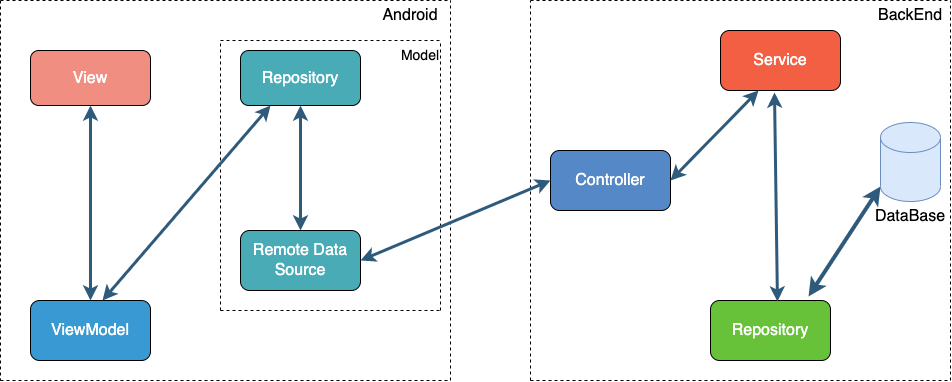
\includegraphics[width=0.85\linewidth]{Figure/sys_architechture.png}
    \caption{Kiến trúc tổng quan của hệ thống}
    \label{fig:use_case_tổng_quan}
\end{figure}
Phần BackEnd của hệ thống được xây dựng bằng Spring boot, dựa trên sự kết hợp của hai mô hình MVC và mô hình ba lớp. Phần Android được xây dựng dựa trên kiến trúc MVVM.  

Ưu điểm khi kết hợp hai mô hình MVC và mô hình ba lớp được sử dụng trong Backend:
\begin{itemize}
    \item Phát triển backend nhanh, đơn giản, dễ lập trình, dễ bảo trì.
    \item Dễ dàng kiểm tra: dễ dàng hơn trong việc kiểm tra, rà soát lỗi do được phân tách một cách độc lập controller, service, repository.
\end{itemize}
Luồng hoạt động của mô hình: Khi người dùng gửi yêu cầu đến server, thì Controller sẽ nhận được request và bắt đầu đi hỏi Service. Service nhận được yêu cầu từ Controller đối với các tính toán đơn giản thì có thể trả về luôn, nhưng đối với  các thao tác liên quan đến Database thì Service thì sẽ liên lạc với Repository để truy cập vào Database truy vấn dữ liệu trả về. Giờ sẽ là cách Server trả ngược lại dữ liệu cho người dùng: Service nhận Entity do Repositoty trả về biến đổi nó cho phù hợp và cuối cùng các Entity được chuyển thành Model và trả về cho Controller. Controller nhận được Model trả về cho App thông qua API.
\newpage
\begin{figure}[H]
    \centering
    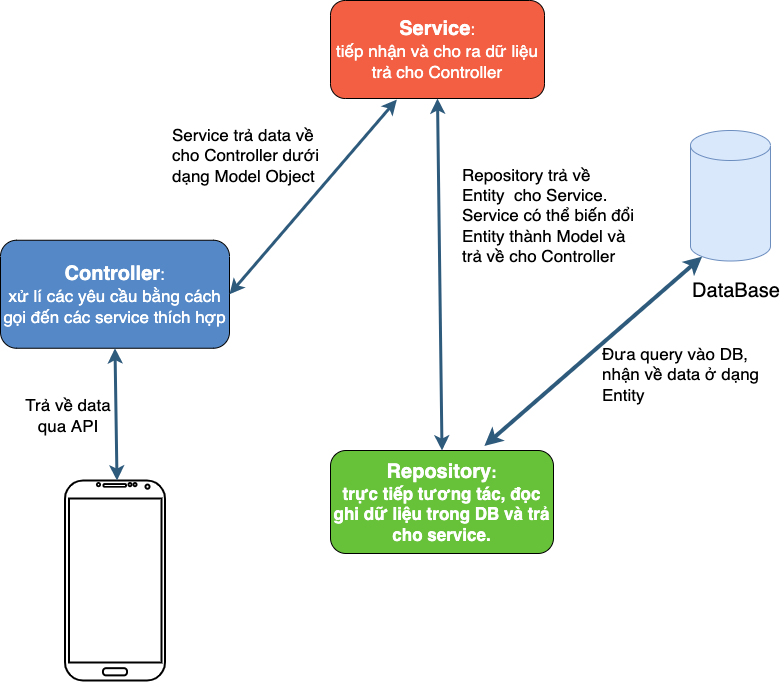
\includegraphics[width=0.75\linewidth]{Figure/backend_architechture.png}
    \caption{Luồng hoạt động của Backend theo mô hình kết hợp giữa mô hình ba lớp và MVC}
    \label{fig:use_case_tổng_quan}
\end{figure}
Mô hình MVVM được phát triển dựa trên cả MVC và MVP. MVVM được phát triển để tách UI ra khỏi logic nghiệp vụ. Một số ưu điểm của MVVM:
\begin{itemize}
 \item Thực hiện Unit test một cách dễ dàng và không phụ thuộc vào View.
 \item Khi test không cần phải tạo mockup như MVP và chỉ cần chỉ cần xác nhận biến observable thích hợp.
 \item Phát triển ứng dụng nhanh, đơn giản, dễ bảo trì.
\end{itemize}
MVVM là một mô hình trong thiết kế xây dựng phần mềm. Ứng dụng được xây dựng dựa trên mô hình MVVM được chia làm 3 phần: Model, View, ViewModel. Các thành phần độc lập với nhau và có một vai trò riêng: 

Model: tầng làm việc với dữ liệu cung cấp cho ứng dụng, tại đây chứa các business logic, được chia làm 2 loại: Local, Remote. Local là nguồn dữ liệu được lấy từ chính thiết bị như cơ sở dũ liệu, bộ nhớ trong, bộ nhớ ngoài, tệp, dữ liệu hệ thống. Remote là các dữ liệu được lấy từ xa như Server, Firebase RealTime database. 

View: Tầng thực hiện nhiệm vụ hiển thị giao diện và tương tác với người dùng. View không chứa dữ liệu mà chỉ cung cấp các phương thức, thuộc tính có tính hiển thị dữ liệu. View chỉ giao tiếp với ViewModel.

ViewModel: có nhiệm vụ xử lí logic của ứng dụng. Giao tiếp với tầng Model nhận dữ liệu tử đây và biến đổi trả về cho View. ViewModel lưu giữ trạng thái của View và điểu khiển việc hiển thị giữ liệu. 

\begin{figure}[H]
    \centering
    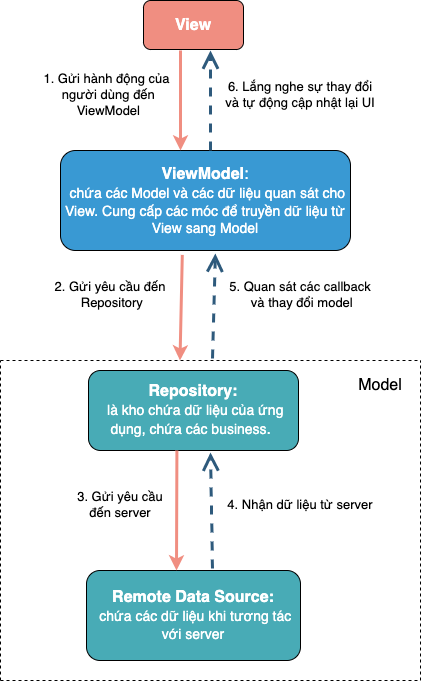
\includegraphics[width=0.75\linewidth]{Figure/android_architechture.png}
    \caption{Luồng hoạt động của Android theo mô hình MVVP}
    \label{fig:use_case_tổng_quan}
\end{figure} \newpage
\subsection{Thiết kế tổng quan} 
\begin{figure}[H]
    \centering
    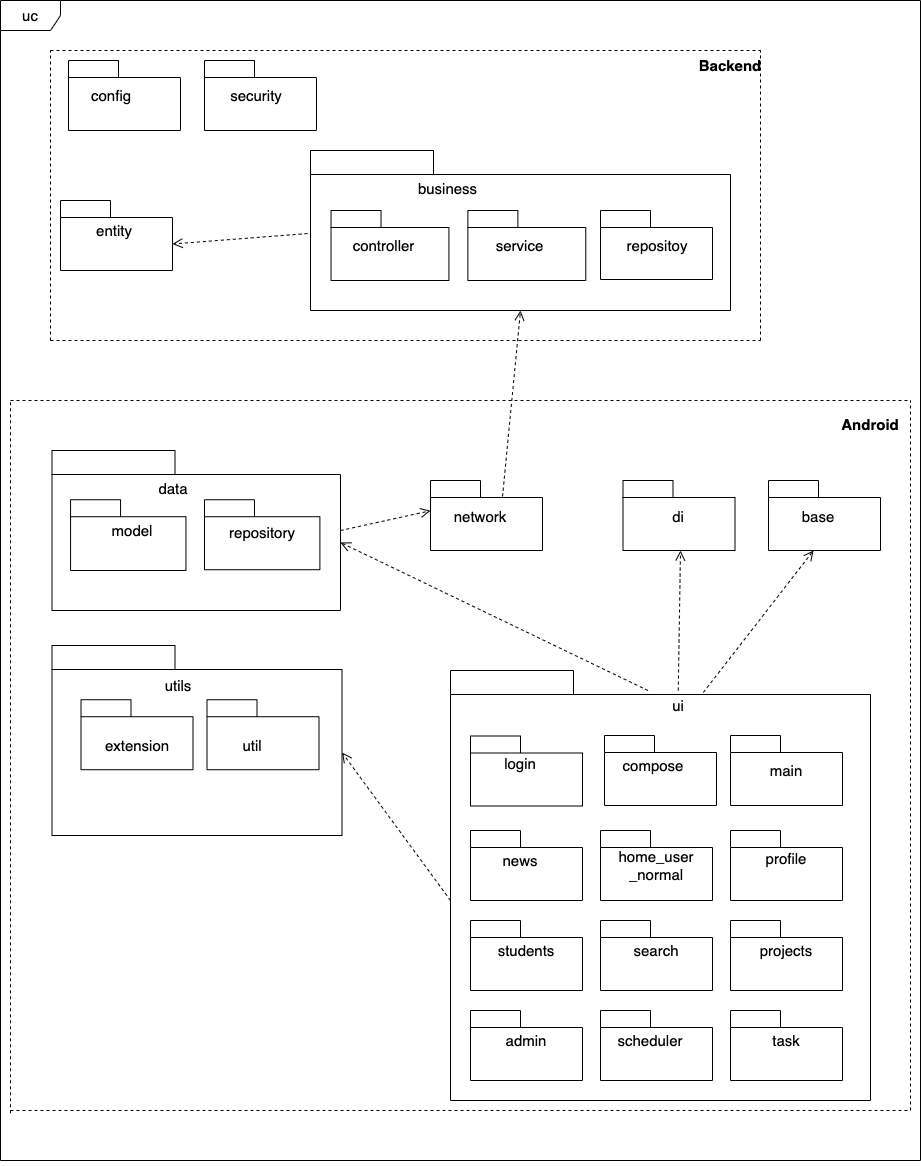
\includegraphics[width=0.95\linewidth]{Figure/package_diagram.png}
    \caption{Thiết kế gói tổng quan}
    \label{fig:use_case_tổng_quan}
\end{figure}
Hệ thống được chia làm 2 phần chính: Backend và Android.

Về phía Backend bao gồm 5 gói chính: (i) config, (ii) security, (iii) entity, (iv) business: 

\textbf{Gói config:} Gói chứa các cấu hình cho spring.

\textbf{Gói security:} Gói chứa các cấu hình liên quan đến Jwt, phân quyền. 

\textbf{Gói entity:} Gói entity tương ứng với các bảng trong cơ sở dữ liệu.

\textbf{Gói business:} Gói chứa các logic của server, nơi xử lí các yêu cầu và trả về kết quả cho ứng dụng.

Về phía Android bao gồm 6 gói chính: (i) di, (ii) base, (iii) data, (iv) utils, (v) network, (vi) ui: 

\textbf{Gói di (Dependency Injection):} Gói chứa các lớp hỗ trợ việc dependency injection giảm thiểu sự phụ thuộc các lớp với nhau. 

\textbf{Gói base:} Gói chứa các lớp cơ bản dùng chung cho nhiều màn hình, được các lớp khác kế thừa và sử dụng.

\textbf{Gói data:} Đại diện cho Model trong kiến trúc MVVM. Cung cấp dữ liệu cho ứng dụng. 

\textbf{Gói network:} Gói chứa các class thực hiện việc giao tiếp với server.

\textbf{Gói utils:} Gói chứa các lớp, các chức năng được tái sử dụng nhiều lần trong hệ thống. 

\textbf{Gói ui (User Interface):} Gói chứa các gói thành phần đại diện cho tầng View trong kiến trúc MVVM. Gói có nhiệm vụ chính là hiển thị dữ liệu và tương tác trực tiếp với người dùng. Bên trong gói ui là các gói thành phần, mỗi gói thành phần bao gồm View, ViewModel. 
\newpage
\subsection{Thiết kế chi tiết gói Task} 
\begin{figure}[H]
    \centering
    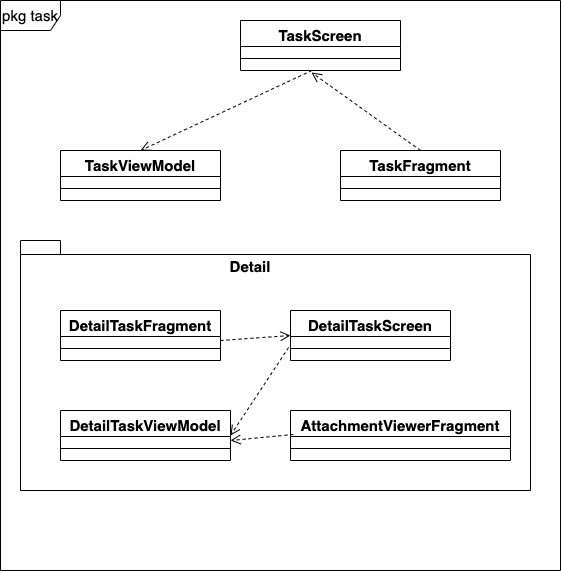
\includegraphics[width=0.75\linewidth]{Figure/package_diagram_task.png}
    \caption{Thiết kế chi tiết gói Task}
    \label{fig:use_case_tổng_quan}
\end{figure}

Hình 4.5 mô tả chi tiết gói Task. Bao gồm các lớp : (i) TaskScreen, (ii) TaskViewModel, (iii) TaskFragment, (iv) DetailTaskFragment, (v) DetailScreen, (vi) DetailTaskViewModel, (viii) AttachmentViewerFragment. Trong đó từng lớp có nhiệm vụ sau:
\begin{itemize}
 \item TaskScreen: Nơi thiết kế giao diện của màn hình danh sách công việc.
 \item TaskViewModel: Nơi nắm giữ dữ liệu về danh sách công việc và thông tin chi tiết về đề tài để lớp TaskFragment hiển thị.
 \item TaskFragment: Màn hình hiển thị danh sách công việc, tên đề tài.
 \item DetailTaskFragment: Màn hình hiển thị chi tiết công việc.
 \item DetailScreen: Nơi thiết kế giao diện cho màn hình chi tiết công việc.
 \item DetailTaskViewModel: Nơi nắm giữ thông tin chi tiết của từng công việc để lớp DetailTaskFragment hiển thị. 
 \item AttachmentViewerFragment: Màn hình hiển thị nội dung file đính kèm. 
\end{itemize} \newpage
\subsection{Thiết kế chi tiết gói Admin} 
\begin{figure}[H]
    \centering
    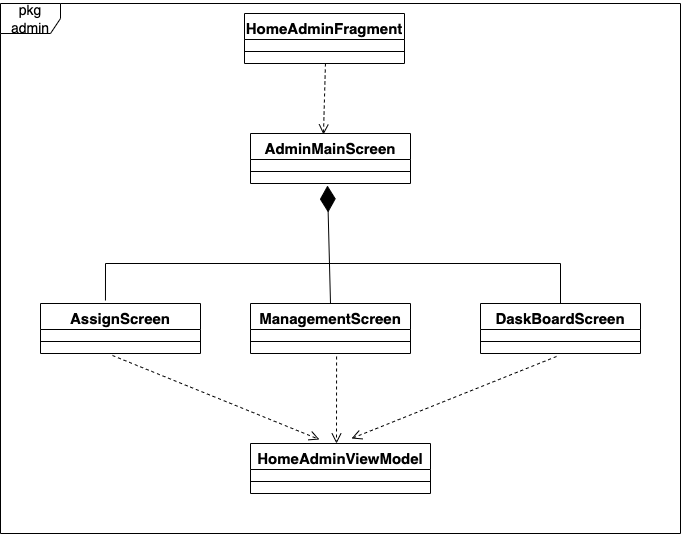
\includegraphics[width=0.75\linewidth]{Figure/package_diagram_admin.png}
    \caption{Thiết kế chi tiết gói Admin}
    \label{fig:use_case_tổng_quan}
\end{figure}
Hình 4.6 mô tả chi tiết gói Admin. Bao gồm các lớp: (i) AdminMainScreen, (ii) AssignScreen, (iii) ManagementScreen, (iv) DashBoardScreen, (v) HomeAdminViewModel, (vi) HomeAdminFragment. Trong đó nhiệm vụ của từng lớp như sau:
\begin{itemize}
    \item AdminScreen: Nơi thiết kế giao diện cho Admin. Màn hình cho admin gồm có 3 tablayout: AssignScreen, ManagementSCreen, DaskBoardScreen.
    \item AssignScreen: Nơi thiết kế màn hình phân công hướng dẫn đồ án.
    \item ManagementScreen: Nơi thiết kế giao diện cho màn hình quản lí danh sách phân công đồ án. 
    \item DashBoardScreen: Nơi thiết kế màn hình thống kê tổng số giảng viên đang được quản lí, tổng số sinh viên đăng kí đồ án. 
    \item HomeAdminViewModel: Nơi nắm giữ dữ liệu về danh sách đồ án, danh sách sinh viên đăng kí từng môn đồ án, danh sách giảng viên, con số thống kê cần có để hiển thị lên màn hình DashBoard.
    \item HomeAdminFragment: Màn hình cha chứa 3 màn hình con: màn hình phân công hướng dẫn đồ án, màn hình quản lí danh sách đồ án, màn hình thống kê. 
\end{itemize}\newpage                                                                                                                              
\subsection{Thiết kế chi tiết gói Projects} 
\begin{figure}[H]
    \centering
    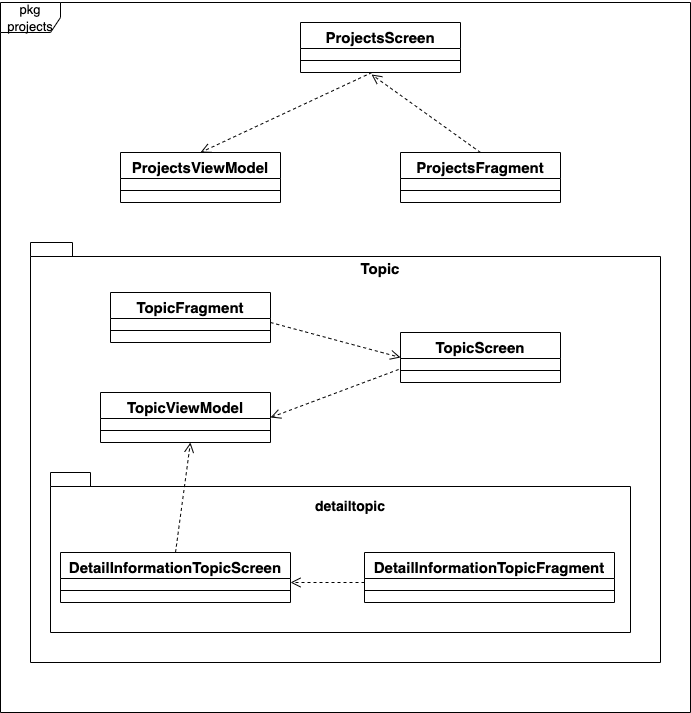
\includegraphics[width=0.75\linewidth]{Figure/package_diagram_projects.png}
    \caption{Thiết kế chi tiết gói Projects}
    \label{fig:use_case_tổng_quan}
\end{figure}
Hình 4.7 mô tả chi tiết gói Projects. Bao gồm các lớp: (i) ProjectsScreen, (ii) ProjectViewModel, (iii) ProjectFragment, (iv) TopicFragment, (v) TopicScreen, (vi) TopicViewModel, (vii) DetailTopicInformationScreen, (viii) DetailTopicInformationFragment. Trong đó nhiệm vụ của từng lớp như sau:
\begin{itemize}
    \item ProjectsScreen: Nơi thiết kế giao diện cho màn hình danh sách đồ án.
    \item ProjectViewModel: Nơi nắm giữ dữ liệu danh sách đồ án, danh sách sinh viên, danh sách các kì học, danh sách giảng viên.
    \item ProjectFragment: Màn hình hiển thị danh sách đồ án hướng dẫn theo kì học.
    \item TopicFragment: Màn hình hiển thị danh sách đề tài của một đồ án. 
    \item TopicScreen: Nơi thiết kế giao diện cho màn hình danh sách đề tài.
    \item TopicViewModel: Nơi nắm giữ danh sách đề tài của một đồ án A để lớp TopicFragment hiển thị.
    \item DetailTopicInformationScreen: Nơi thiết kế giao diện cho màn hình thông tin chi tiết về đề tài: tên đề tài, mô tả đề tài, thông tin giảng viên hướng dẫn, thông tin sinh viên thực hiện, thời gian thực hiện.
    \item DetailTopicInformationFragment: Màn hình hiển thị thông tin chi tiết về đề tài. 
\end{itemize}
\section{Thiết kế chi tiết}
\subsection{Thiết kế giao diện}
Đối với việc phát triển ứng dụng thì thiết kế giao diện là đặc biệt quan trọng. Thiết kế giao diện quyết định đến hiệu năng tương tác người dùng và dựa trên một số yếu tố sau:

Kích thước màn hình: ứng dụng được thiết kế phù hợp với tất cả các loại điện thoại thông minh và phổ biến hiện nay. Không thực hiện fix cứng các thống số trên màn hình. Giao diện được thiết kế trên điện thoại Galaxy S10+(1440 x 3040).

Màu sắc: Ứng dụng có sự thống nhất về màu sắc, chỉ sử dụng hai màu chủ đạo là màu đỏ và trắng. 

Độ phân giải: Hỗ trợ tốt nhất với các ứng dụng có độ phân giải HD trở lên. 

Thiết kế nút: Sử dụng các icon tượng hình. Các icon được cung cập bởi Google và một số icon được lấy từ trang Icon8. Tất cả các icon đều tuân theo chuẩn Material Dessign cả về màu sắc lẫn kích thước. 

\subsection{Thiết kế lớp}
\subsubsection{Thiết kế chi tiết lớp Task}
Thiết kế chi tiết lớp Task được miêu tả như hình 4.8. Ở đây lớp TaskViewModel phụ thuộc vào TaskScreenState. TaskScreenState chứa danh sách TaskData đại hiện cho công việc cần hiển thị và danh sách các công việc khi thực hiện lọc theo status thông quan hàm filterTaskByStatus(). Lớp TaskViewModel cần thực hiện công việc lấy ra danh sách công việc của topic qua phương thức findAllTaskByIdTopic().

Lớp TaskScreen cần các tham số đầu vào là TaskViewModel để bind dữ liệu vào trong các Compose. Và sau đó để hiển thị danh sách công việc lên màn hình,  TaskScreen sẽ được TaskFragment gọi qua hàm onCreateView() để vẽ UI lên màn hình. Hàm initArg() trong TaskFragment để lấy ra dữ liệu khi chuyển từ một màn hình A đến màn hình TaskFragment. 

Lớp DetailTaskScreen chứa các Compose để vẽ nên giao diện hoàn chỉnh cho màn hình DetaiTaskFragment như DetailTask(), BottomBarAttachment(), CommentSection(). 
Lớp DetailTaskViewModel chứa phương thức getDetailTask() để lấy thông tin chi tiết của công việc hiển thị lên màn hình chi tiết công việc và phương thức getComment() để lấy về toàn bộ bình luận có trong màn hình này. Khi tạo mới một công việc hay chỉnh sửa một công việc thì các công việc sẽ được lưu lại thông qua hàm saveTask() ở ViewModel. Khi có bất cứ sự thay đổi nào về thông tin chi tiết của công việc thì ngay lập tức DetailTaskFragment sẽ được cập nhật và người dùng nhận được thông tin đã cập nhật trong tức thì. Lớp AttachmentViewerFragment gọi đến ViewModel và lấy ra tên file đính kèm, sau đó sử dụng WebViewContainer một Compose Android cung cấp sẵn để hiển thị file. 

\begin{figure}[H]
    \centering
    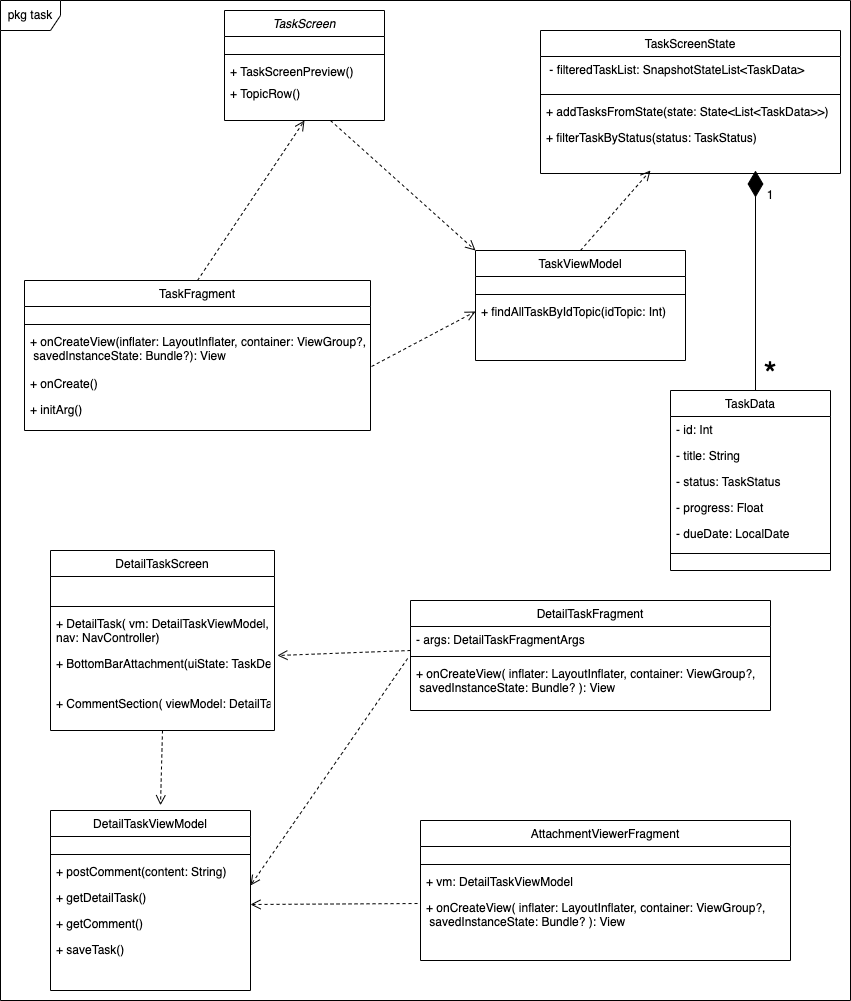
\includegraphics[width=0.95\linewidth]{Figure/chi_tiet_lop_task.png}
    \caption{Thiết kế chi tiết lớp Task}
    \label{fig:use_case_tổng_quan}
\end{figure}
\subsubsection{Thiết kế chi tiết lớp Admin} 
Thiết kế chi tiết lớp Task được miêu tả như hình 4.9. Ở đây lớp AdminMainScreen là nơi thiết kế giao diện cho admin, quy định khi nào chuyển đến các lớp DashBoardScreen, ManagementScreen, AssignScreen. Các lớp DashBoardScreen, ManagementScreen, AssignScreen phụ thuộc vào HomeAdminViewModel. HomeAdminViewModel có chứa HomeScreenState khi state thay đổi thì nội dung trong DashBoardScreen, ManagementScreen, AssignScreen tự động cập nhật theo.

HomeViewModel chứa các hàm getAllCurrentSemester() để lấy danh sách các kì học, hàm getInformationDashBoard() để lấy thông tin cho DashBoardScreen, hàm fetchDataManagementScreen() để đổ dữ liệu vào cho lớp ManagementScreen,  hàm fetchDataAssignScreen() để đổ dữ liệu vào cho lớp AssignScreen, hàm onSubmit() thực hiện phân công hướng dẫn đồ án. Hàm deleteItemChecked() thực hiện xoá danh sách phân công được chọn. 

Lớp HomeAdminFragment gọi đến lớp AdminMainScreen trong hàm onCreateView() để vẽ UI lên màn hình. Token được lưu trong SharedPreference sẽ được xoá khi người dùng đăng xuất ra khỏi hệ thống.
\newpage
\begin{figure}[H]
    \centering
    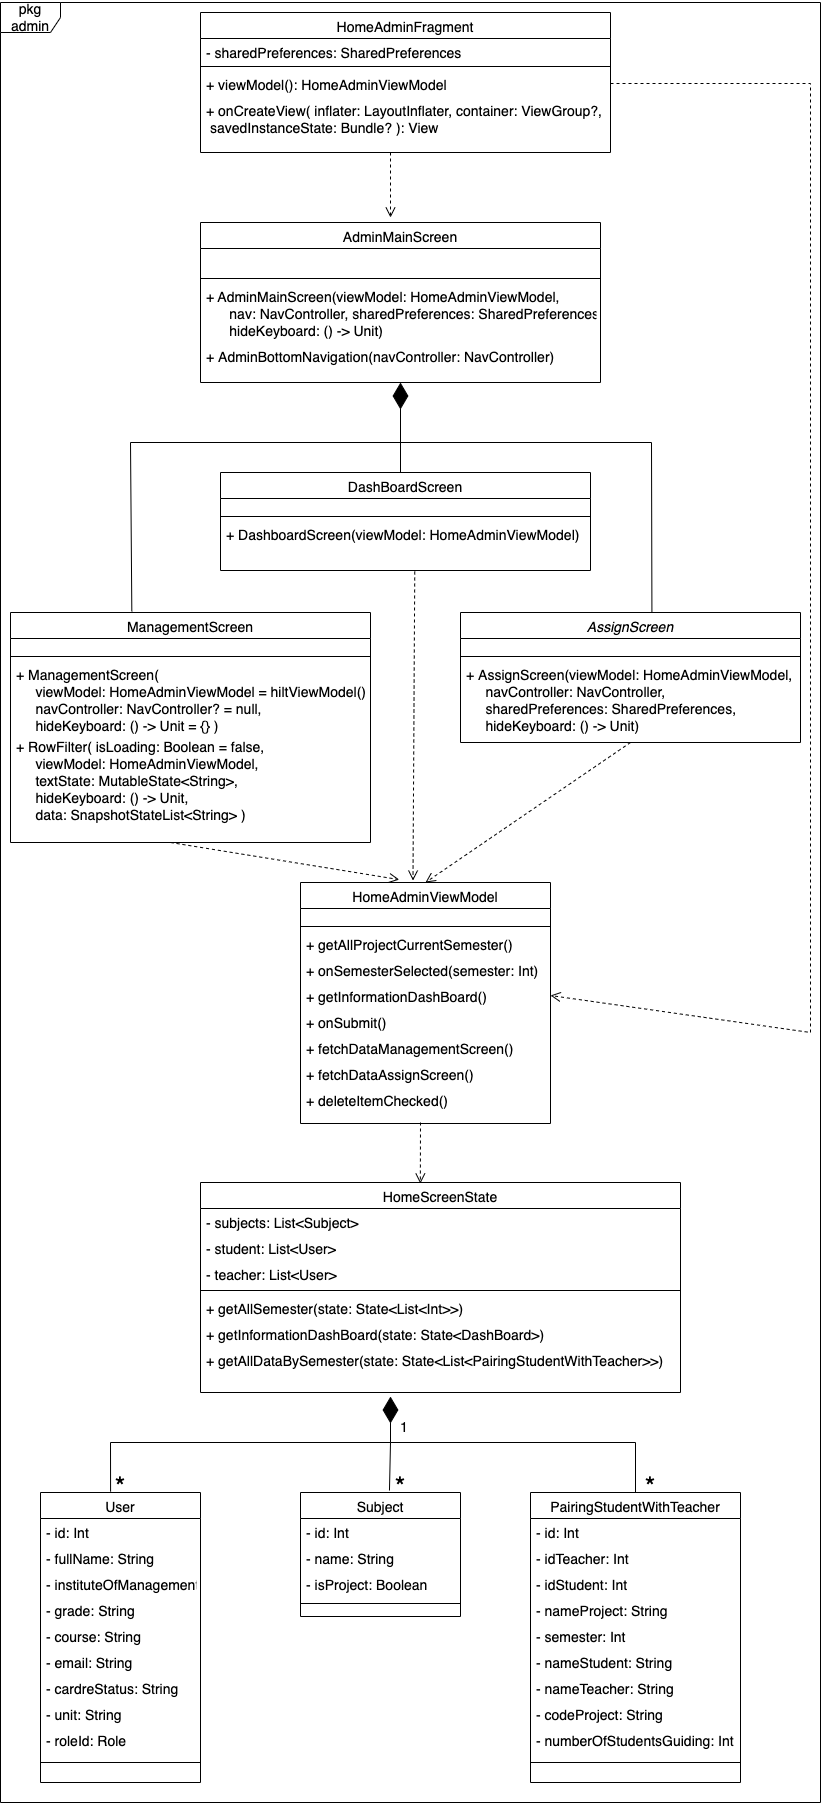
\includegraphics[width=0.76\linewidth]{Figure/chi_tiet_lop_admin (1).png}
    \caption{Thiết kế chi tiết lớp Admin}
    \label{fig:use_case_tổng_quan}
\end{figure}\newpage
\subsection{Thiết kế cơ sở dữ liệu}
\begin{figure}[H]
    \centering
    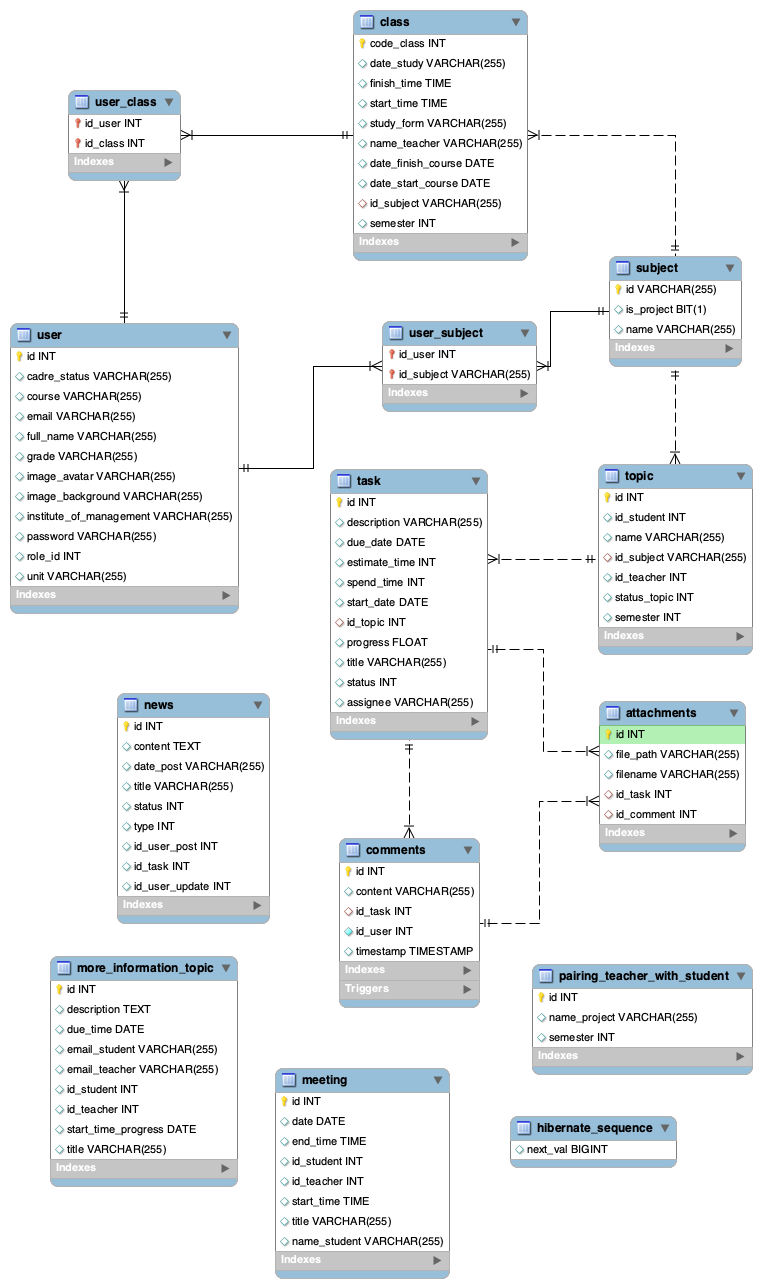
\includegraphics[width=0.8\linewidth]{Figure/Untitled.png}
    \caption{Sơ đồ thiết kế cơ sở dữ liệu}
    \label{fig:use_case_tổng_quan}
\end{figure}
\newpage
\textbf{Bảng dữ liệu User}

Mục đích: Lưu thông tin của người dùng.

Danh sách thuộc tính: 
\begin{table}[H]
\centering
\bgroup
\renewcommand{\arraystretch}{1.5}%
\begin{tabular}{|L{0.2\linewidth}|L{0.2\linewidth}|L{0.22\linewidth}|L{0.1\linewidth}|L{0.15\linewidth}|}
\hline
\textbf{Tên} & \textbf{Kiểu dữ liệu} & \textbf{Mô tả} & \textbf{Có bắt buộc} & \textbf{Có Ràng buộc} \\ \hline
id & Int & Id của người dùng & có & Khóa chính \\ \hline
password & Varchar(255) & Mật khẩu của người dùng & có &  \\ \hline
full\_name & Varchar(255) & Tên đầy đủ của người dùng & có &  \\ \hline
email & Varchar(255) & Email của  người dùng & có & Duy nhất \\ \hline
course & Varchar(255) & Nếu là sinh viên thì thuộc khóa bao nhiêu & Không &  \\ \hline
grade & Varchar(255) & Lớp & không &  \\ \hline
cadre\_status & Varchar(255) & Nếu là giảng viên thì trạng thái cán bộ là gì & Không &  \\ \hline
institute\_of \_management & Varchar(255) & Khoa/ viện quản lí & Có &  \\ \hline
image\_avatar & Varchar(255) & Tên file làm ảnh đại diện & Không &  \\ \hline
image\_background & Varchar(255) & Tên file làm ảnh bìa & Không &  \\ \hline
unit & Varchar(255) & Chương trình học & Có &  \\ \hline
role\_id & Int & Role\_id = 1  ứng với phân quyền của quản trị viên.  Role\_id\ = 2 ứng với  phân quyền của giảng viên. Role\_id = 3 ứng với phân quyền của sinh viên. & Có &  \\ \hline
\end{tabular}
\egroup
\caption{Bảng dữ liệu User}
\end{table}

\textbf{Bảng dữ liệu Class}

Mục đích: Lưu thông tin lớp học. 

Danh sách thuộc tính:
\begin{table}[H]
\centering
\bgroup
\renewcommand{\arraystretch}{1.5}%
\begin{tabular}{|L{0.2\linewidth}|L{0.18\linewidth}|L{0.22\linewidth}|L{0.1\linewidth}|L{0.15\linewidth}|}
\hline
\textbf{Tên} & \textbf{Kiểu dữ liệu} & \textbf{Mô tả} & \textbf{Có bắt  buộc} & \textbf{Có Ràng buộc} \\ \hline
code\_class & Int & Mã môn học & Có & Khóa chính \\ \hline
date\_study & Varchar(255) & Ngày học môn học này trong tuần: Thứ hai, hay ba... & Có &  \\ \hline
finish\_time & Time & Giờ kết thúc môn học & Có &  \\ \hline
start\_time & Time & Giờ bắt đầu môn học & Có &  \\ \hline
study\_form & Varchar(255) & Hình thức học: online  hay offline & Không &  \\ \hline
name\_teacher & Varchar(255) & Tên giảng viên giảng dạy & Không &  \\ \hline
\begin{tabular}[c]{@{}l@{}}date\_finish\\ \_course\end{tabular} & Date & Ngày kết thúc môn học & Không &  \\ \hline
\begin{tabular}[c]{@{}l@{}}date\_start\\ \_course\end{tabular} & Date & Ngày bắt đầu môn học & Có &  \\ \hline
id\_subject & Varchar(255) & Mã môn học & Có & Khoá ngoại \\ \hline
semester & Int & Học kì & Có &  \\ \hline
\end{tabular}
\egroup
\caption{Bảng dữ liệu Class}
\end{table}
\newpage
\textbf{Bảng dữ liệu User\_class}

Mục đích: Bảng trung gian để bẻ mối quan hệ nhiều nhiều giữa User, Class thành hai quan hệ một nhiều.

Danh sách thuộc tính: 
\begin{table}[H]
\centering
\bgroup
\renewcommand{\arraystretch}{1.5}%
\begin{tabular}{|L{0.2\linewidth}|L{0.18\linewidth}|L{0.22\linewidth}|L{0.1\linewidth}|L{0.15\linewidth}|}
\hline
\textbf{Tên} & \textbf{Kiểu dữ liệu} & \textbf{Mô tả} & \textbf{\begin{tabular}[c]{@{}l@{}}Có bắt\\  buộc\end{tabular}} & \textbf{\begin{tabular}[c]{@{}l@{}}Có Ràng\\ buộc\end{tabular}} \\ \hline
id\_user & Int & Id của người dùng & Có & Khóa chính \\ \hline
id\_class & Int & Id lớp học & Có & Khoá chính \\ \hline
\end{tabular}
\egroup
\caption{Bảng dữ liệu User\_class}
\end{table}
\textbf{Bảng dữ liệu News}

Mục đích: Lưu thông tin thông báo

Danh sách thuộc tính: 
\begin{table}[H]
\centering
\bgroup
\renewcommand{\arraystretch}{1.5}%
\begin{tabular}{|L{0.2\linewidth}|L{0.18\linewidth}|L{0.22\linewidth}|L{0.1\linewidth}|L{0.15\linewidth}|}
\hline
\textbf{Tên} & \textbf{Kiểu dữ liệu} & \textbf{Mô tả} & \textbf{Có bắt buộc} & \textbf{Có Ràng buộc} \\ \hline
id & Int & Id thông báo & Có & Khóa chính \\ \hline
title & Text & Tên thông báo & Có &  \\ \hline
content & Varchar(255) & Nội dung thông báo & Có &  \\ \hline
date\_post & Varchar(255) & Ngày đăng thông báo & Có &  \\ \hline
status & Int & Trạng thái thông báo: 0: Chưa đọc 1: Đã đọc & Có &  \\ \hline
type & Int & Loại thông báo: 0: Thông báo thường 1: Thông báo về đồ án & Không &  \\ \hline
id\_task & Int & Id công việc & Không &  \\ \hline
id\_user\_update & Int &Id người cập nhật công việc & Không &  \\ \hline
\end{tabular}
\egroup
\caption{Bảng dữ liệu News}
\end{table} 

\newpage
\textbf{Bảng dữ liệu User\_subject}

Mục đích: Bảng trung gian để bẻ mối quan hệ nhiều nhiều giữa User, Subject thành hai quan hệ một nhiều.

Danh sách thuộc tính:
\begin{table}[H]
\centering
\bgroup
\renewcommand{\arraystretch}{1.5}%
\begin{tabular}{|L{0.2\linewidth}|L{0.18\linewidth}|L{0.22\linewidth}|L{0.1\linewidth}|L{0.15\linewidth}|}
\hline
\textbf{Tên} & \textbf{Kiểu dữ liệu} & \textbf{Mô tả} & \textbf{Có bắt buộc} & \textbf{Có Ràng buộc} \\ \hline
id\_user & Int & Id của người dùng & Có & Khóa chính \\ \hline
id\_subject & Varchar(255) & Mã môn học & Có & Khoá chính \\ \hline
\end{tabular}
\egroup
\caption{Bảng dữ liệu User\_subject}
\end{table}

\textbf{Bảng dữ liệu Task}

Mục đích: Lưu thông tin công việc.

Danh sách thuộc tính:
\begin{table}[H]
\centering
\bgroup
\renewcommand{\arraystretch}{1.5}%
\begin{tabular}{|L{0.2\linewidth}|L{0.18\linewidth}|L{0.22\linewidth}|L{0.1\linewidth}|L{0.15\linewidth}|}
\hline
\textbf{Tên} & \textbf{Kiểu dữ liệu} & \textbf{Mô tả} & \textbf{Có bắt  buộc} & \textbf{Có Ràng buộc} \\ \hline
id & Int & Mã môn học & Có & Khóa chính \\ \hline
title & Varchar(255) & Tên công việc & Có &  \\ \hline
desciption & Varchar(255) & Mô tả chi tiết công việc & Không &  \\ \hline
due\_date & Date & Hạn hoàn thành công việc & Có &  \\ \hline
start\_date & Date & Thời gian có thể bắt đầu công việc & Có &  \\ \hline
estimate\_time & Int & Số giờ dự đoán hoàn thành & Có &  \\ \hline
progress & Float & Tiến độ công việc & Có &  \\ \hline
status & Int & Trạng thái công việc & Có &  \\ \hline
\begin{tabular}[c]{@{}l@{}}name\_user\\ \_create\end{tabular} & Varchar(255) & Tên người tạo công việc & Có &  \\ \hline
id\_topic & Int & Id đề tài & Có & Khoá ngoại \\ \hline
\end{tabular}
\egroup
\caption{Bảng dữ liệu Task}
\end{table}

\textbf{Bảng dữ liệu Topic}

Mục đích: Lưu thông tin của đề tài.

Danh sách thuộc tính:
\begin{table}[H]
\centering
\bgroup
\renewcommand{\arraystretch}{1.5}%
\begin{tabular}{|L{0.2\linewidth}|L{0.18\linewidth}|L{0.22\linewidth}|L{0.1\linewidth}|L{0.15\linewidth}|}
\hline
\textbf{Tên} & \textbf{Kiểu dữ liệu} & \textbf{Mô tả} & \textbf{Có bắt buộc} & \textbf{Có Ràng buộc} \\ \hline
id & Int & Id đề tài & Có & Khóa chính \\ \hline
id\_student & Int & Id của sinh viên & Có &  \\ \hline
name & Varchar(255) & Tên đề tài & Có &  \\ \hline
id\_subject & Varchar(255) & Mã môn học & Có & Khoá ngoại \\ \hline
id\_teacher & Int & Thời gian có thể bắt đầu công việc & Có &  \\ \hline
status\_topic & Int & Trạng thái của đề tài( Đã được chấp nhận, hay đang yêu cầu) & Có &  \\ \hline
semester & Int & Học kì & Có &  \\ \hline
\end{tabular}
\egroup
\caption{Bảng dữ liệu Topic}
\end{table}

\textbf{Bảng dữ liệu Comments}

Mục đích: Lưu thông tin của bình luận.

Danh sách thuộc tính:
\begin{table}[H]
\centering
\bgroup
\renewcommand{\arraystretch}{1.5}%
\begin{tabular}{|L{0.2\linewidth}|L{0.18\linewidth}|L{0.22\linewidth}|L{0.1\linewidth}|L{0.15\linewidth}|}
\hline
\textbf{Tên} & \textbf{Kiểu dữ liệu} & \textbf{Mô tả} & \textbf{Có bắt buộc} & \textbf{Có Ràng buộc} \\ \hline
id & Int & Id đề tài & Có & Khóa chính \\ \hline
content & Varchar(255) & Nội dung hình luận & Có &  \\ \hline
id\_task & Int & Id công việc & Có & Khoá ngoại \\ \hline
id\_user & Int & Id người bình luận & Có &  \\ \hline
timestamp & TIMESTAMP & Thời gian bình luận & Có &  \\ \hline
\end{tabular}
\egroup
\caption{Bảng dữ liệu Comments}
\end{table}

\textbf{Bảng dữ liệu Meeting}

Mục đích: Lưu thông tin chi tiết về lịch gặp mặt của sinh viên và giảng viên.

Danh sách thuộc tính: 
\begin{table}[H]
\centering
\bgroup
\renewcommand{\arraystretch}{1.5}%
\begin{tabular}{|L{0.2\linewidth}|L{0.18\linewidth}|L{0.22\linewidth}|L{0.1\linewidth}|L{0.15\linewidth}|}
\hline
\textbf{Tên} & \textbf{Kiểu dữ liệu} & \textbf{Mô tả} & \textbf{Có bắt buộc} & \textbf{Có Ràng buộc} \\ \hline
id & Int & Id cuộc gặp giữa sinh viên và giảng viên & Có & Khóa chính \\ \hline
date & Date & Ngày gặp & Có &  \\ \hline
title & Varchar(255) & Nội dung gặp mặt & Có &  \\ \hline
name\_student & Varchar(255) & Tên sinh viên gặp & Có &  \\ \hline
id\_teacher & Timestamp & Id giảng viên & Có &  \\ \hline
id\_student & Int & Id sinh viên & Có &  \\ \hline
start\_time & Time & Thời gian bắt đầu & Có &  \\ \hline
end\_time & Time & Thời gian kết thúc & Có &  \\ \hline
\end{tabular}
\egroup
\caption{Bảng dữ liệu Meeting}
\end{table}

\textbf{Bảng dữ liệu Attachments}

Mục đích: Lưu thông tin file đính kèm

Danh sách thuộc tính:
\begin{table}[H]
\centering
\bgroup
\renewcommand{\arraystretch}{1.5}%
\begin{tabular}{|L{0.2\linewidth}|L{0.18\linewidth}|L{0.22\linewidth}|L{0.1\linewidth}|L{0.15\linewidth}|}
\hline
\textbf{Tên} & \textbf{Kiểu dữ liệu} & \textbf{Mô tả} & \textbf{Có bắt buộc} & \textbf{Có Ràng buộc} \\ \hline
id & Int & Id file đính kèm & Có & Khóa chính \\ \hline
file\_path & Varchar(255) & UUID của file & Có &  \\ \hline
file\_name & Varchar(255) & Tên file & Có &  \\ \hline
id\_task & Int & Id task & Có & Khoá ngoại \\ \hline
id\_comment & Int & Id bình luận & Có & Khoá ngoại \\ \hline
\end{tabular}
\egroup
\caption{Bảng dữ liệu Attachments}
\end{table}
\newpage
\textbf{Bảng dữ liệu More\_information\_topic}

Mục đích: Lưu thông tin chi tiết của đề tài.

Danh sách thuộc tính:
\begin{table}[H]
\centering
\bgroup
\renewcommand{\arraystretch}{1.5}%
\begin{tabular}{|L{0.2\linewidth}|L{0.18\linewidth}|L{0.22\linewidth}|L{0.1\linewidth}|L{0.15\linewidth}|}
\hline
\textbf{Tên} & \textbf{Kiểu dữ liệu} & \textbf{Mô tả} & \textbf{Có bắt buộc} & \textbf{Có Ràng buộc} \\ \hline
id & Int & Id của đề tài & Có & Khóa chính \\ \hline
desciption & Varchar(255) & Mô tả chi tiết đề tài & Có &  \\ \hline
title & Varchar(255) & Tên đề tài & Có &  \\ \hline
\begin{tabular}[c]{@{}l@{}}start\_time\\ \_progress\end{tabular} & Date & Thời gian bắt đầu thực hiện đồ án & Có &  \\ \hline
due\_time & Date & Thời gian kết thúc đồ án & Có &  \\ \hline
id\_student & Int & Id sinh viên & Có &  \\ \hline
id\_teacher & Int & Id giảng viên & Có &  \\ \hline
email\_student & Varchar(255) & Email sinh viên & Có &  \\ \hline
process\_score & Float & Điểm quá trình của đồ án môn học & Không & \\ \hline
end\_score & Float & Điểm cuối kì của đồ án môn học & Không &  \\ \hline
state\_process & Int & Trạng thái của đồ án tốt nghiệp là Đang thực hiện hay đã hoàn thành, hay chưa hoàn thành & Không &  \\ \hline
\end{tabular}
\egroup
\caption{Bảng dữ liệu More\_information\_topic}
\end{table} 
\newpage
\textbf{Bảng dữ liệu Pairing\_teacher\_with\_student}

Mục đích: Lưu thông tin phân hướng dẫn công đồ án.

Danh sách thuộc tính:

\begin{table}[H]
\centering
\bgroup
\renewcommand{\arraystretch}{1.5}%
\begin{tabular}{|L{0.2\linewidth}|L{0.18\linewidth}|L{0.22\linewidth}|L{0.1\linewidth}|L{0.15\linewidth}|}
\hline
\textbf{Tên} & \textbf{Kiểu dữ liệu} & \textbf{Mô tả} & \textbf{Có bắt buộc} & \textbf{Có Ràng buộc} \\ \hline
id & Int &Id ghép đôi giữa giảng viên và sinh viên & Có & Khóa chính \\ \hline
name\_project & Varchar(255) & Tên đồ án & Có &  \\ \hline
semester & Int & Học kì & Có &  \\ \hline
id\_student & Int & Id sinh viên & Có &  \\ \hline
id\_teacher & Int & Id giảng viên & Có &  \\ \hline
\end{tabular}
\egroup
\caption{Bảng dữ liệu Pairing\_teacher\_with\_student}
\end{table}


\textbf{Bảng dữ liệu Subject}

Mục đích: Lưu thông tin môn học.

Danh sách thuộc tính:
\begin{table}[H]
\centering
\bgroup
\renewcommand{\arraystretch}{1.5}%

\begin{tabular}{|L{0.1\linewidth}|L{0.18\linewidth}|L{0.32\linewidth}|L{0.1\linewidth}|L{0.15\linewidth}|}
\hline
\textbf{Tên} & \textbf{Kiểu dữ liệu} & \textbf{Mô tả} & \textbf{Có bắt  buộc} & \textbf{Có Ràng buộc} \\ \hline
id & Varchar(255) & Mã môn học & Có & Khóa chính \\ \hline
type & Int & Có phải môn đồ án hay không. Type = 0 ứng với môn học bình thường. Type = 1 ứng với đồ án môn học. Type = 2 ứng với đồ án tốt nghiệp & Có &  \\ \hline
name & Varchar(255) & Tên môn học & Có &  \\ \hline
\end{tabular}

\egroup
\caption{Bảng dữ liệu Subject}
\end{table}

\section{Xây dựng ứng dụng}
\subsection{Thư viện và công cụ sử dụng}
Các thư viện và công cụ sử dụng để xây dựng "Ứng dụng quản lí đồ án trên nền tảng Android": \newpage
\begin{table}[H]
\centering
\bgroup
\renewcommand{\arraystretch}{1.6}%

\begin{tabular}{|L{0.25\linewidth}|L{0.3\linewidth}|L{0.3\linewidth}|}
\hline
\textbf{Công cụ} & \textbf{Mục đích} & \textbf{Địa chỉ URL} \\ \hline
Android Studio & IDE lập trình & https://developer.android. -com/studio \\ \hline
Intellij & IDE lập trình & https://www.jetbrains. com/idea \\ \hline
MYSQL & Hệ quản trị cơ sở dữ liệu & https://www.mysql.com \\ \hline
Kotlin & Ngôn ngữ lập trình server và Android& https://kotlinlang.org/ \\ \hline
Spring boot & Framework lập trình phía server & https://spring.io/ \\ \hline
Kotlin compose & Xây dựng giao diện & https://developer.android. com/jetpack/compose \\ \hline
Coroutines & Thư viện hỗ trợ lập trình bất đồng bộ & https://developer.android. com/kotlin/coroutines \\ \hline
Dagger Hilt & Thư viện hỗ trợ lập trình & https://developer.android. com/training/dependency-injection/hilt-android \\ \hline
Json web token & Xác thực và phân quyền & https://jwt.io/introduction \\ \hline
Docker & Tạo môi trường chạy spring boot & https://www.docker.com/ 101-tutorial/ \\ \hline
Minio Object storage & Server lưu trữ các file đính kèm & https://min.io  \\ \hline
Azure cloud & Dịch vụ cloud deploy backend &  \\ \hline
\end{tabular}

\egroup
\caption{Danh sách thư viện và công cụ sử dụng}
\end{table}

\newpage
\subsection{Kết quả đạt được} 
\begin{table}[H]
\centering
\bgroup
\renewcommand{\arraystretch}{1.6}%

\begin{tabular}{|l|l|}
\hline
\textbf{Mô tả} & \textbf{Thông tin} \\ \hline
Số dòng code & 19821 \\ \hline
Số lượng lớp & 185 \\ \hline
Số giao diện & 22 \\ \hline
Dung lượng mã nguồn và tài nguyên & 318MB \\ \hline
Công cụ kiểm thử & JUnit \\ \hline
Môi trường lập trình & MacOS \\ \hline
\end{tabular}

\egroup
\caption{Thông tin kết quả đạt được}
\end{table}
\subsection{Minh hoạ các chức năng chính}
Kết quả đạt được là xây dựng thành công một ứng dụng quản lí đồ án trên nền tảng Android với các chức năng cơ bản:

Sinh viên và giảng viên sau khi đăng nhập có thể xem lịch ngày hôm nay, xem thông báo tin tức quan trọng từ trường, tạo công việc, chỉnh sửa công việc, bình luận công việc. Ngoài ra sinh viên còn có thể tra cứu thông tin sinh viên, giảng viên, lớp học, danh sách lớp, xem thời khoá biểu; giảng viên sẽ nhận được thông báo ngay sau khi sinh viên cập nhật công việc, có thể tạo lịch gặp với sinh viên, xem danh sách đồ án hướng dẫn theo kì và xem thông tin chi tiết các đề tài. 

Với quản trị viên, quản trị viên có thể phân công hướng dẫn đồ án, xoá một phân công hướng dẫn bất kì nếu thấy không hợp lí, lọc danh sách phân công đồ án theo kì học, tên giảng viên, tên sinh viên, tên đồ án, thống kê tổng số sinh viên đăng kí học các môn đồ án, số giảng viên đang được quản lí tại học kì hiện tại. 

Hình ảnh minh hoạ sử dụng ứng dụng:

\textbf{*Đối với người dùng là sinh viên hoặc giảng viên:} \newpage

\begin{figure}[H]
\begin{minipage}{0.5\textwidth}
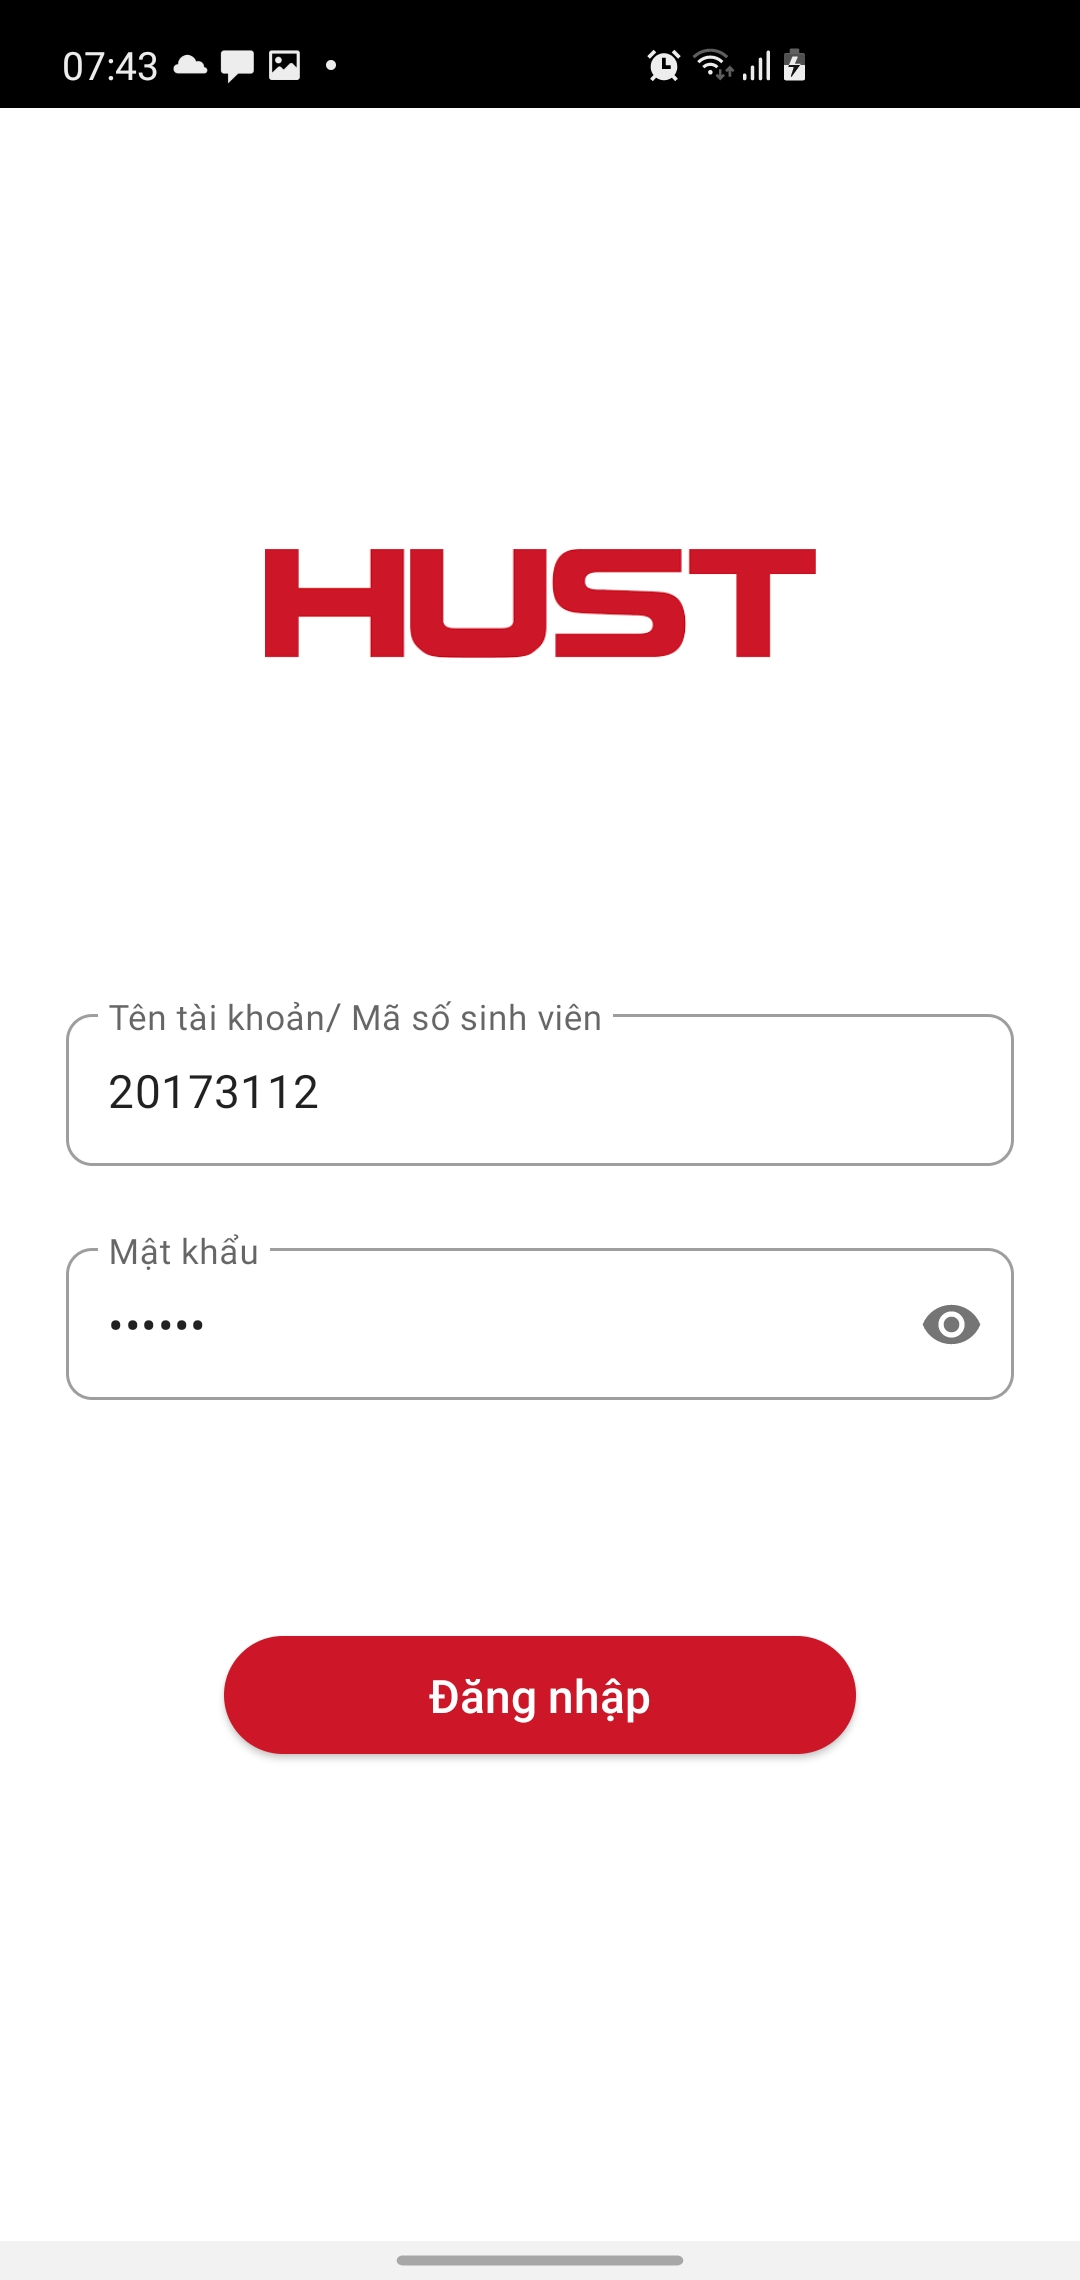
\includegraphics[width=0.7\linewidth]{Figure/screen/screen_login.jpg}
\caption{Màn hình đăng nhập} \label{fig:screen_login}
\end{minipage}
\hspace{\fill}
\begin{minipage}{0.5\textwidth}
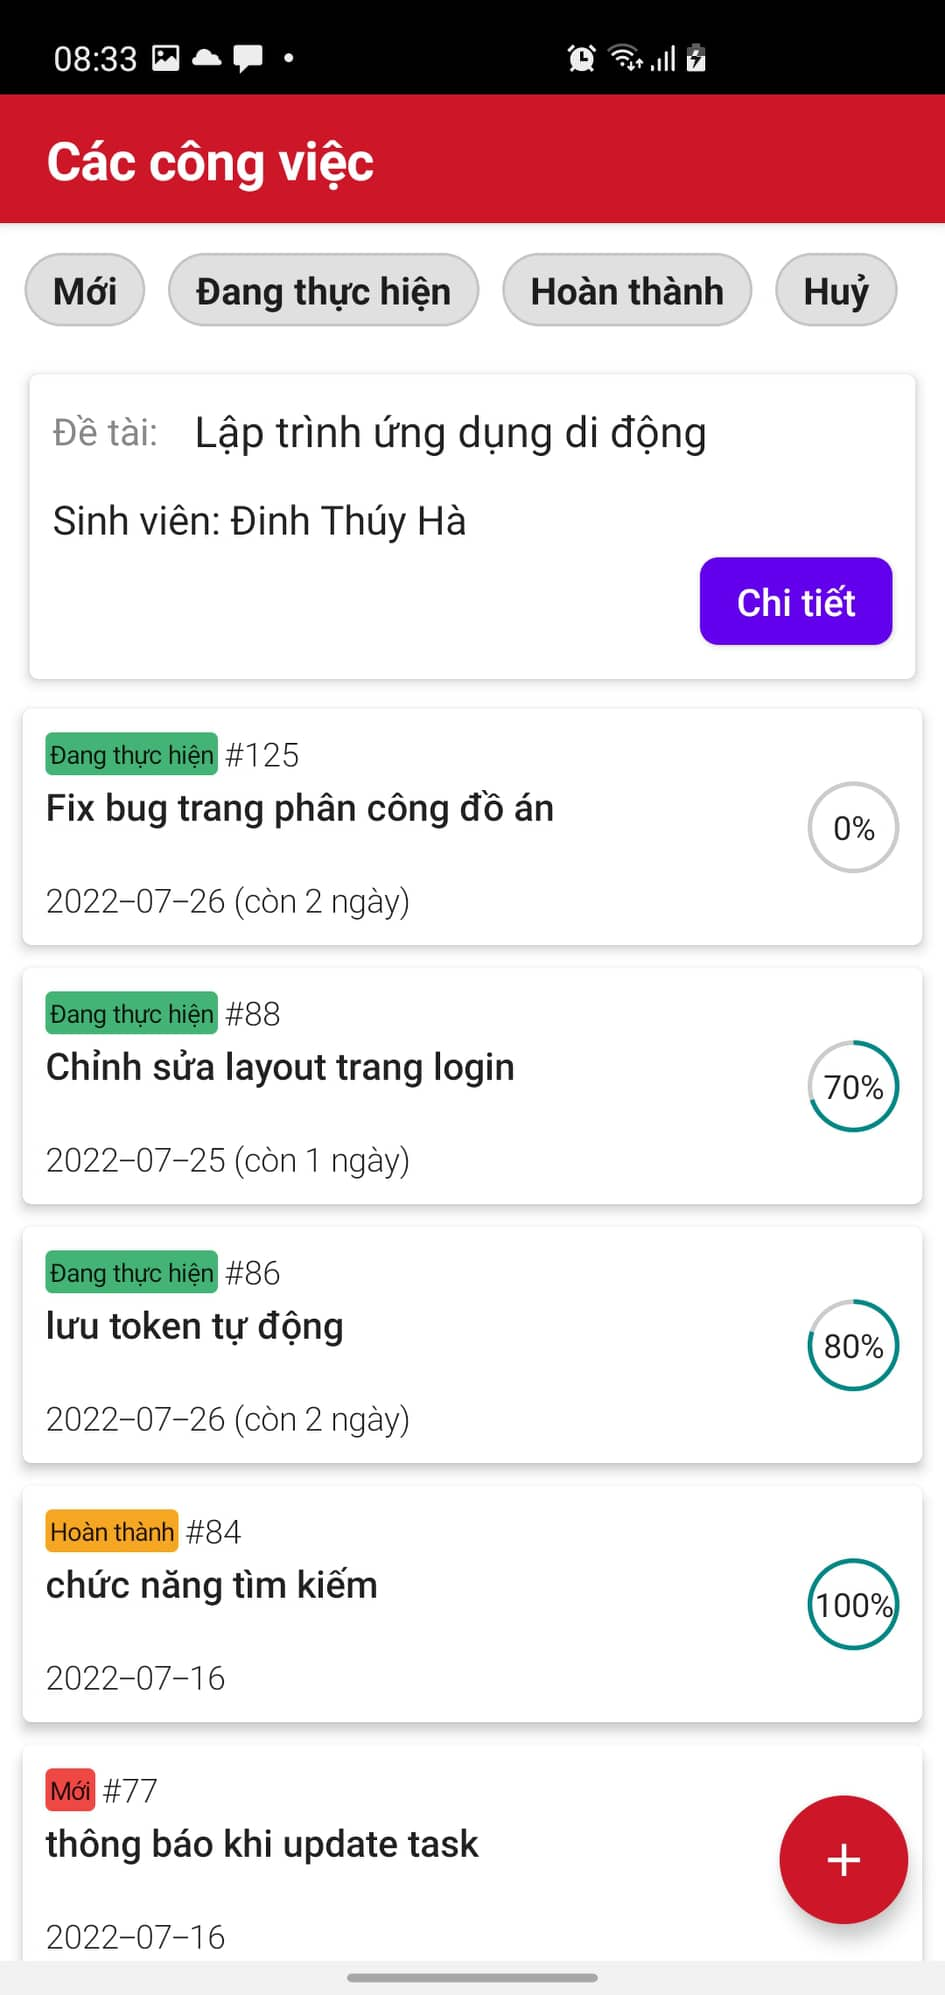
\includegraphics[width=0.7\linewidth]{Figure/screen/list_task.jpeg}
\caption{Màn hình danh sách công việc} \label{fig:list_task}
\end{minipage}
\end{figure}

%% a non-floating version
\noindent %  override any \parindent effect
\begin{minipage}{0.5\textwidth}
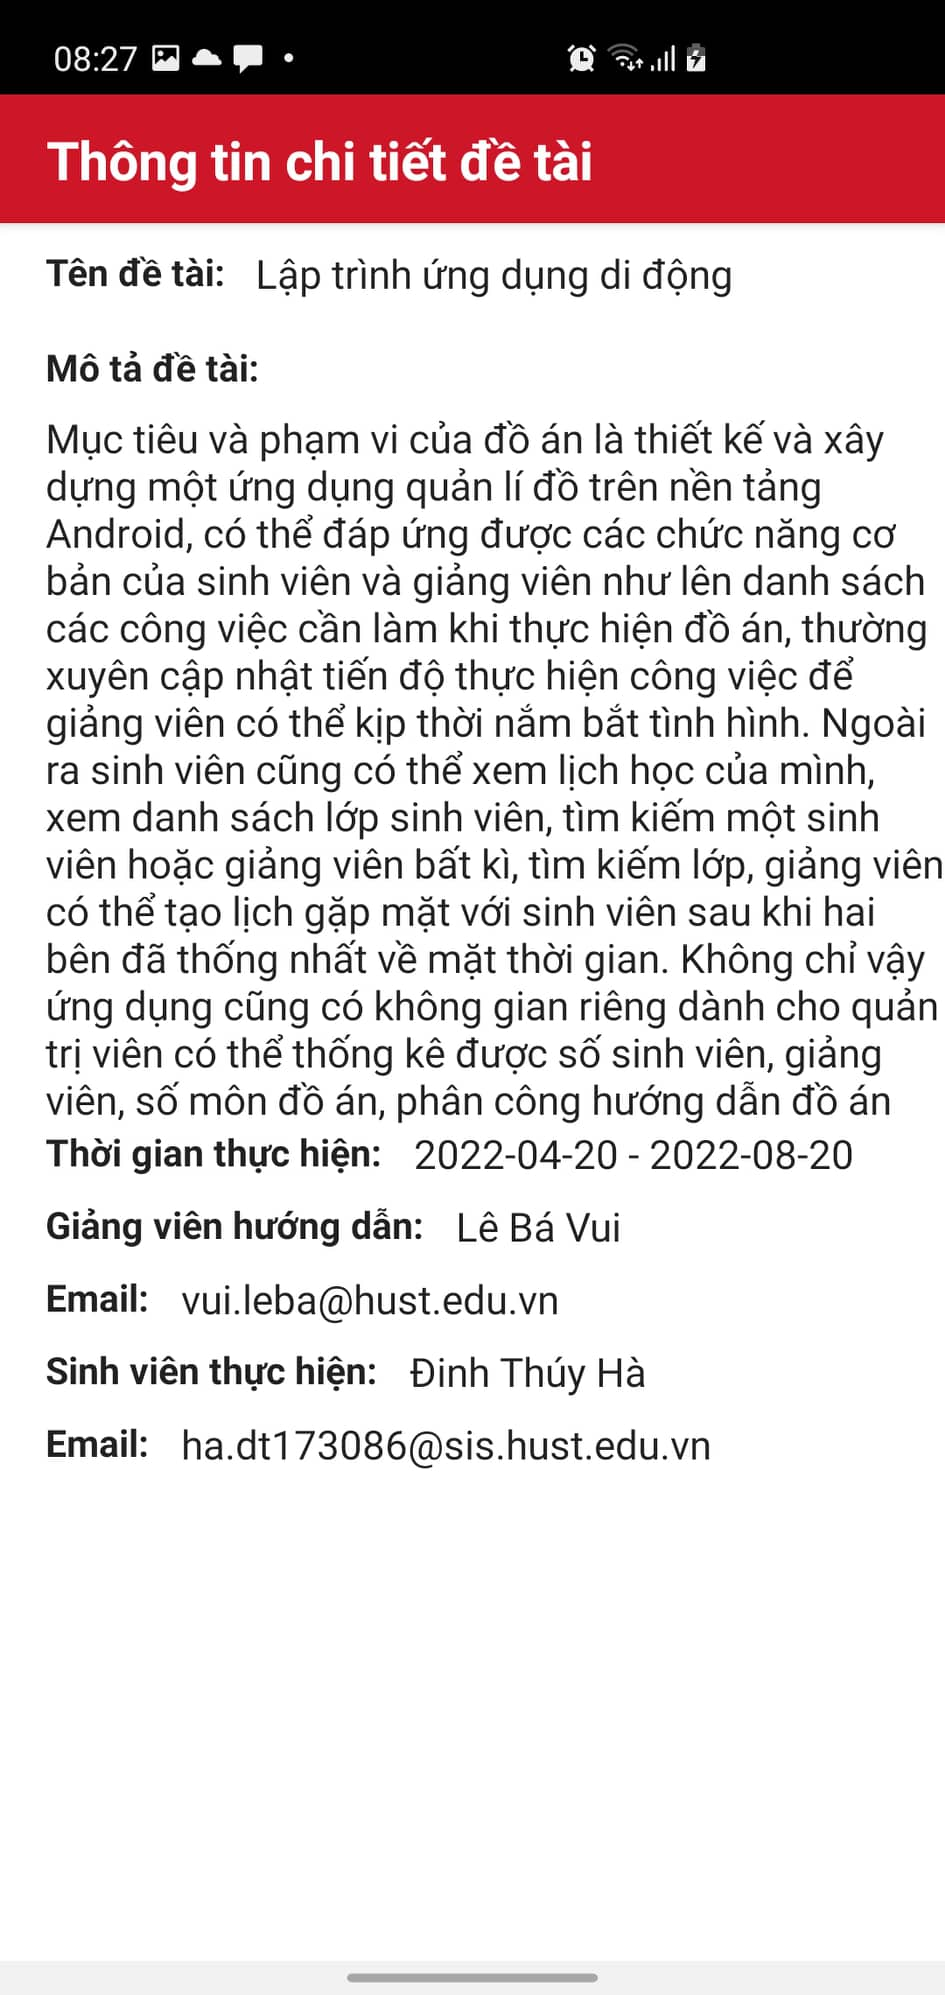
\includegraphics[width=0.70\linewidth]{Figure/screen/information_topic.jpeg}
\captionof{figure}{Màn hình xem chi tiết đề tài} \label{fig:information_topic}
\end{minipage}
\hspace{\fill}
\begin{minipage}{0.5\textwidth}
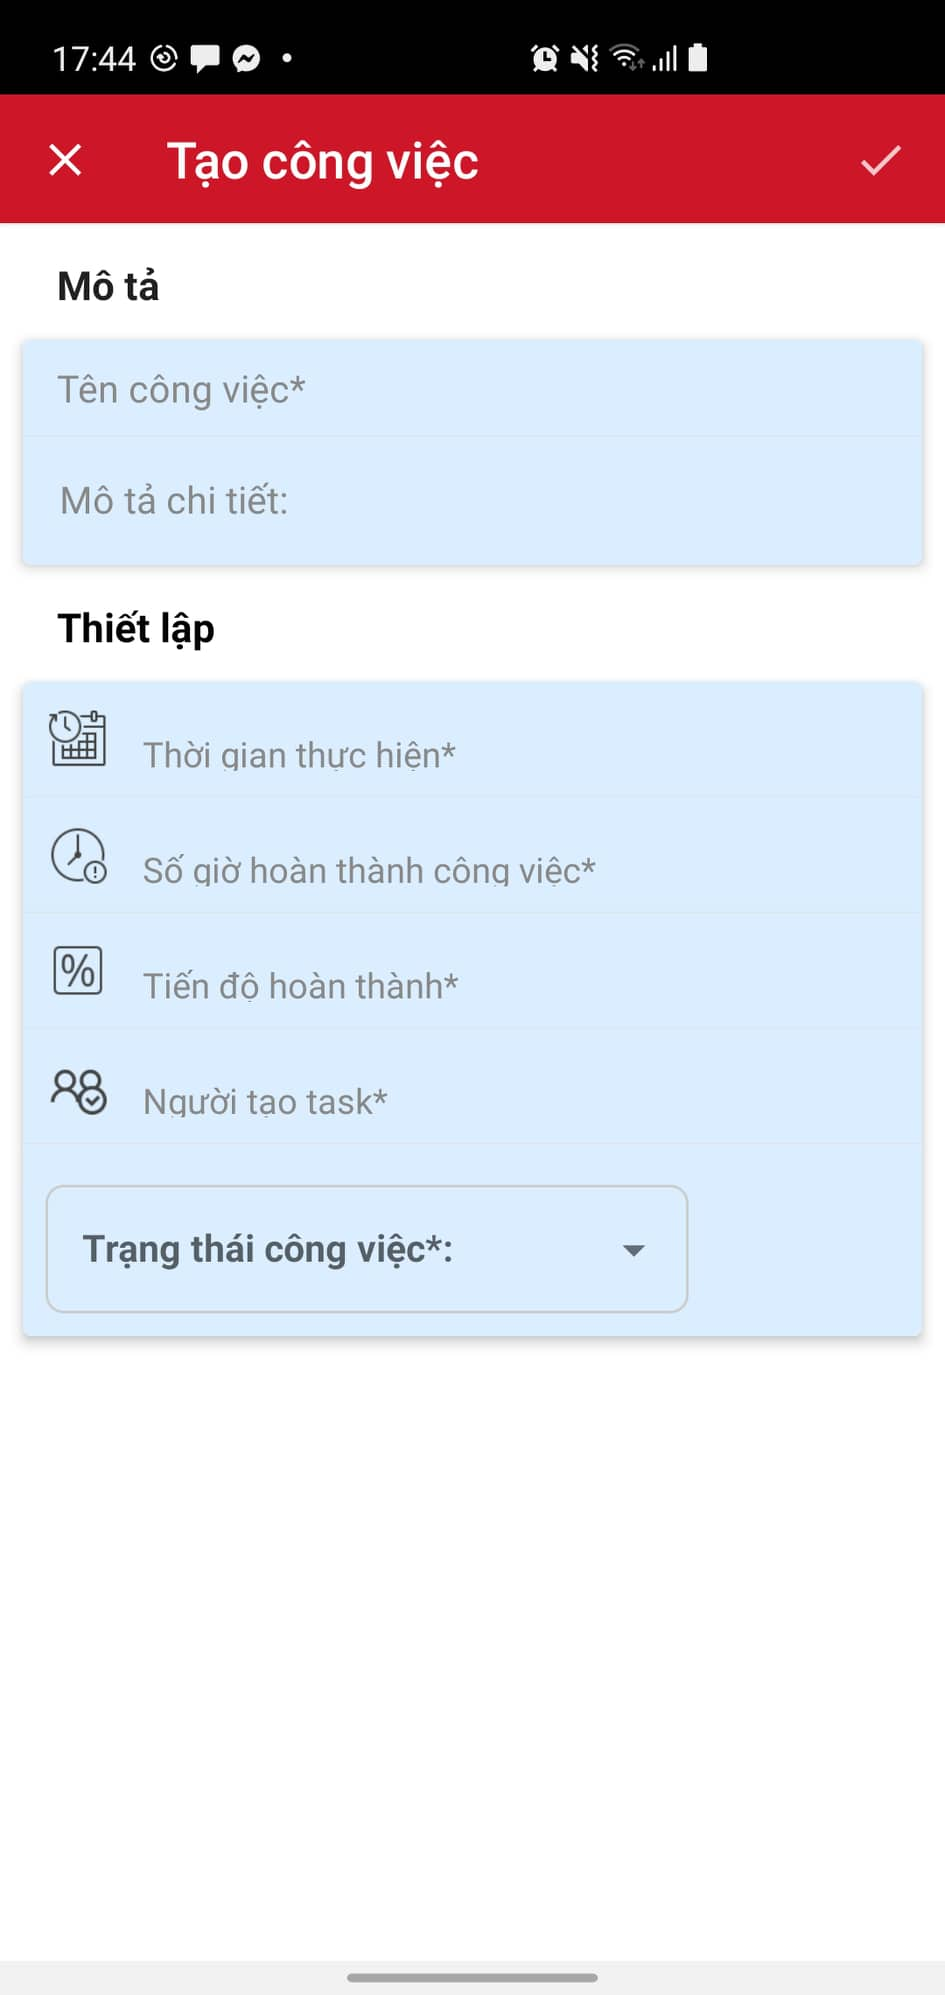
\includegraphics[width=0.70\linewidth]{Figure/screen/new_task.jpg}
\captionof{figure}{Màn hình tạo công việc} \label{fig:star2}
\end{minipage}
\caption{Màn hình tạo công việc} \label{fig:screen_login}

\begin{figure}[H]
\begin{minipage}{0.5\textwidth}
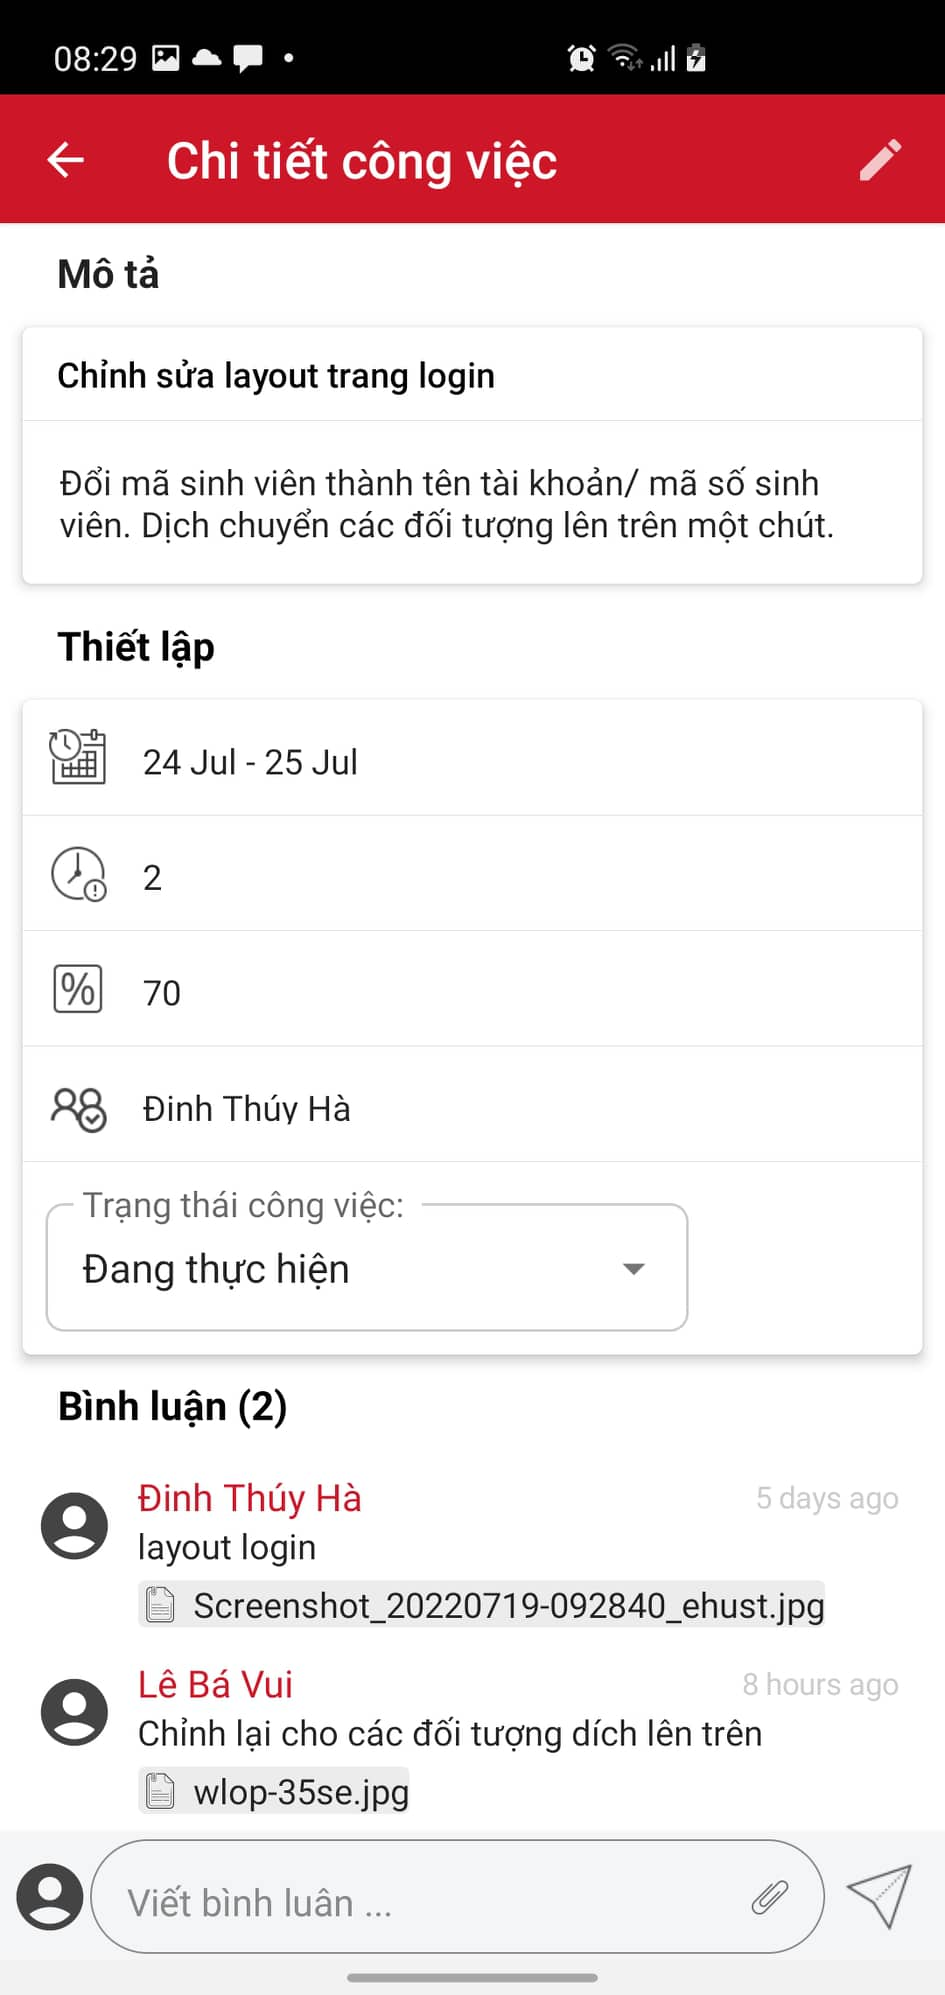
\includegraphics[width=0.7\linewidth]{Figure/screen/detail_task.jpeg}
\caption{Màn hình chi tiết công việc} \label{fig:screen_login}
\end{minipage}
\hspace{\fill}
\begin{minipage}{0.5\textwidth}
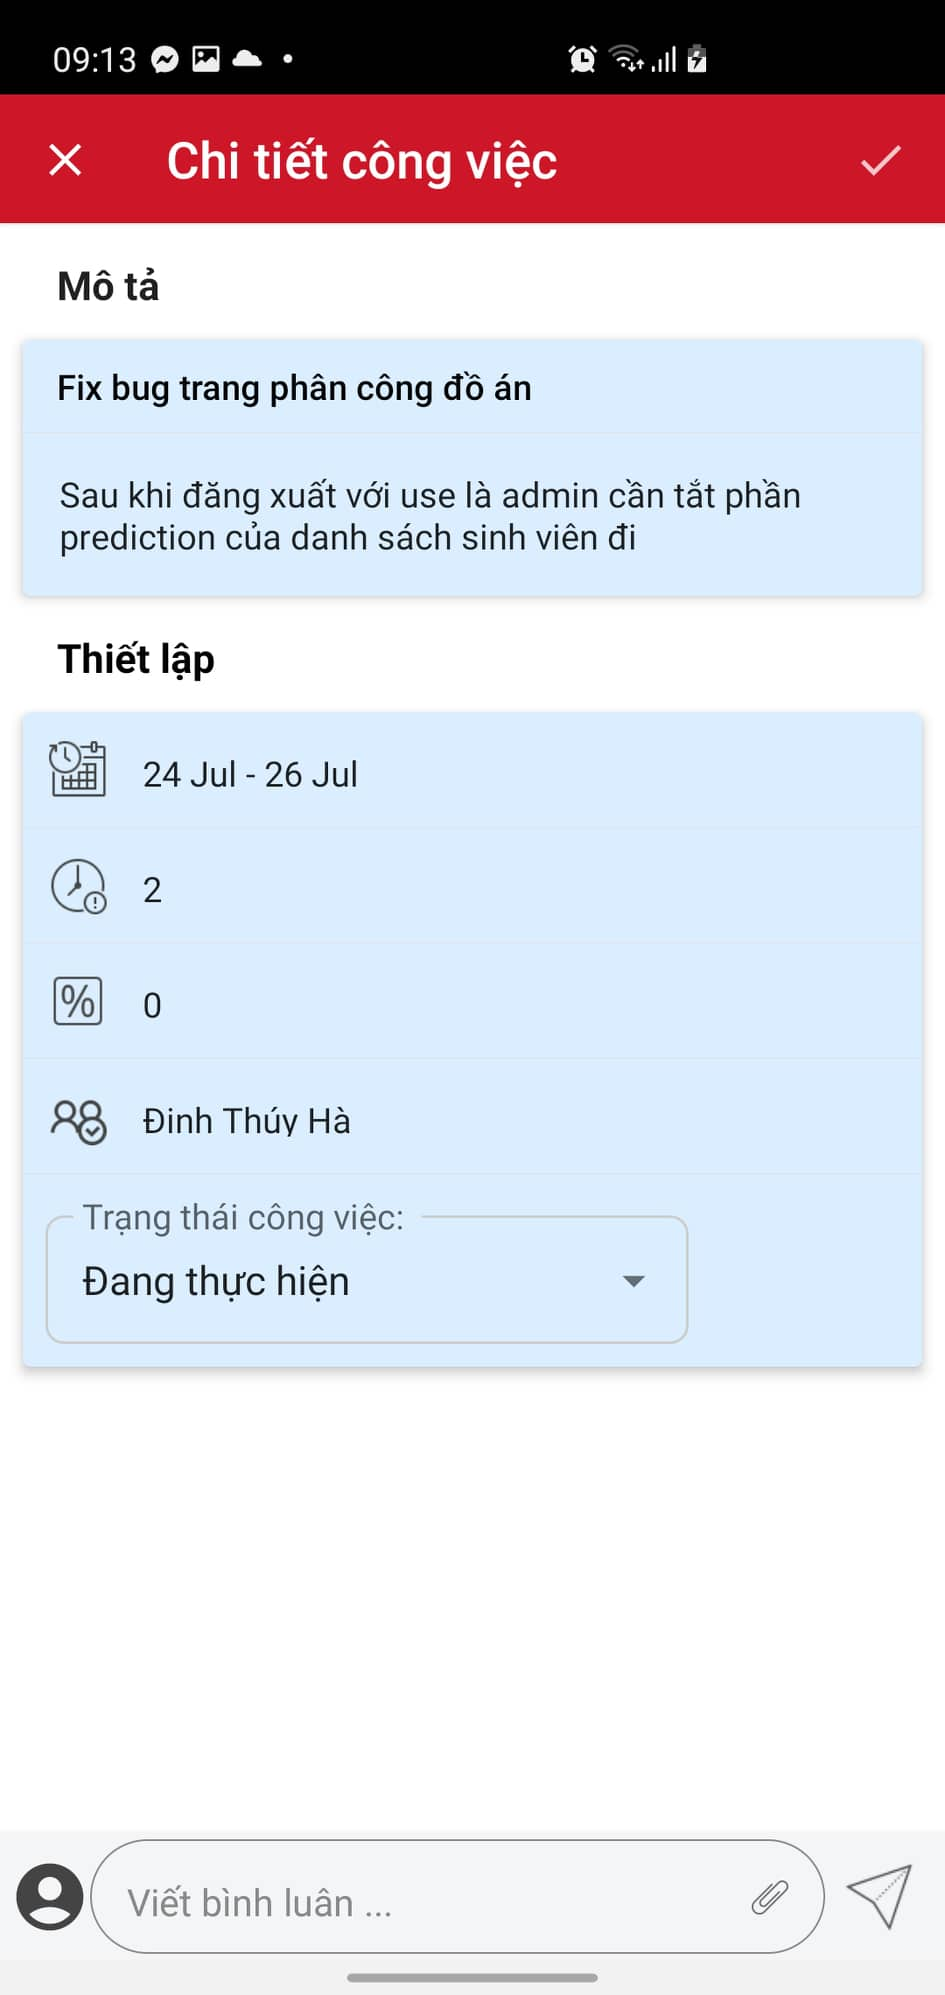
\includegraphics[width=0.7\linewidth]{Figure/screen/edit_task.jpeg}
\caption{Màn hình chỉnh sửa công việc} \label{fig:list_task}
\end{minipage}
\end{figure}
%% a non-floating version
\noindent %  override any \parindent effect
\begin{minipage}{0.5\textwidth}
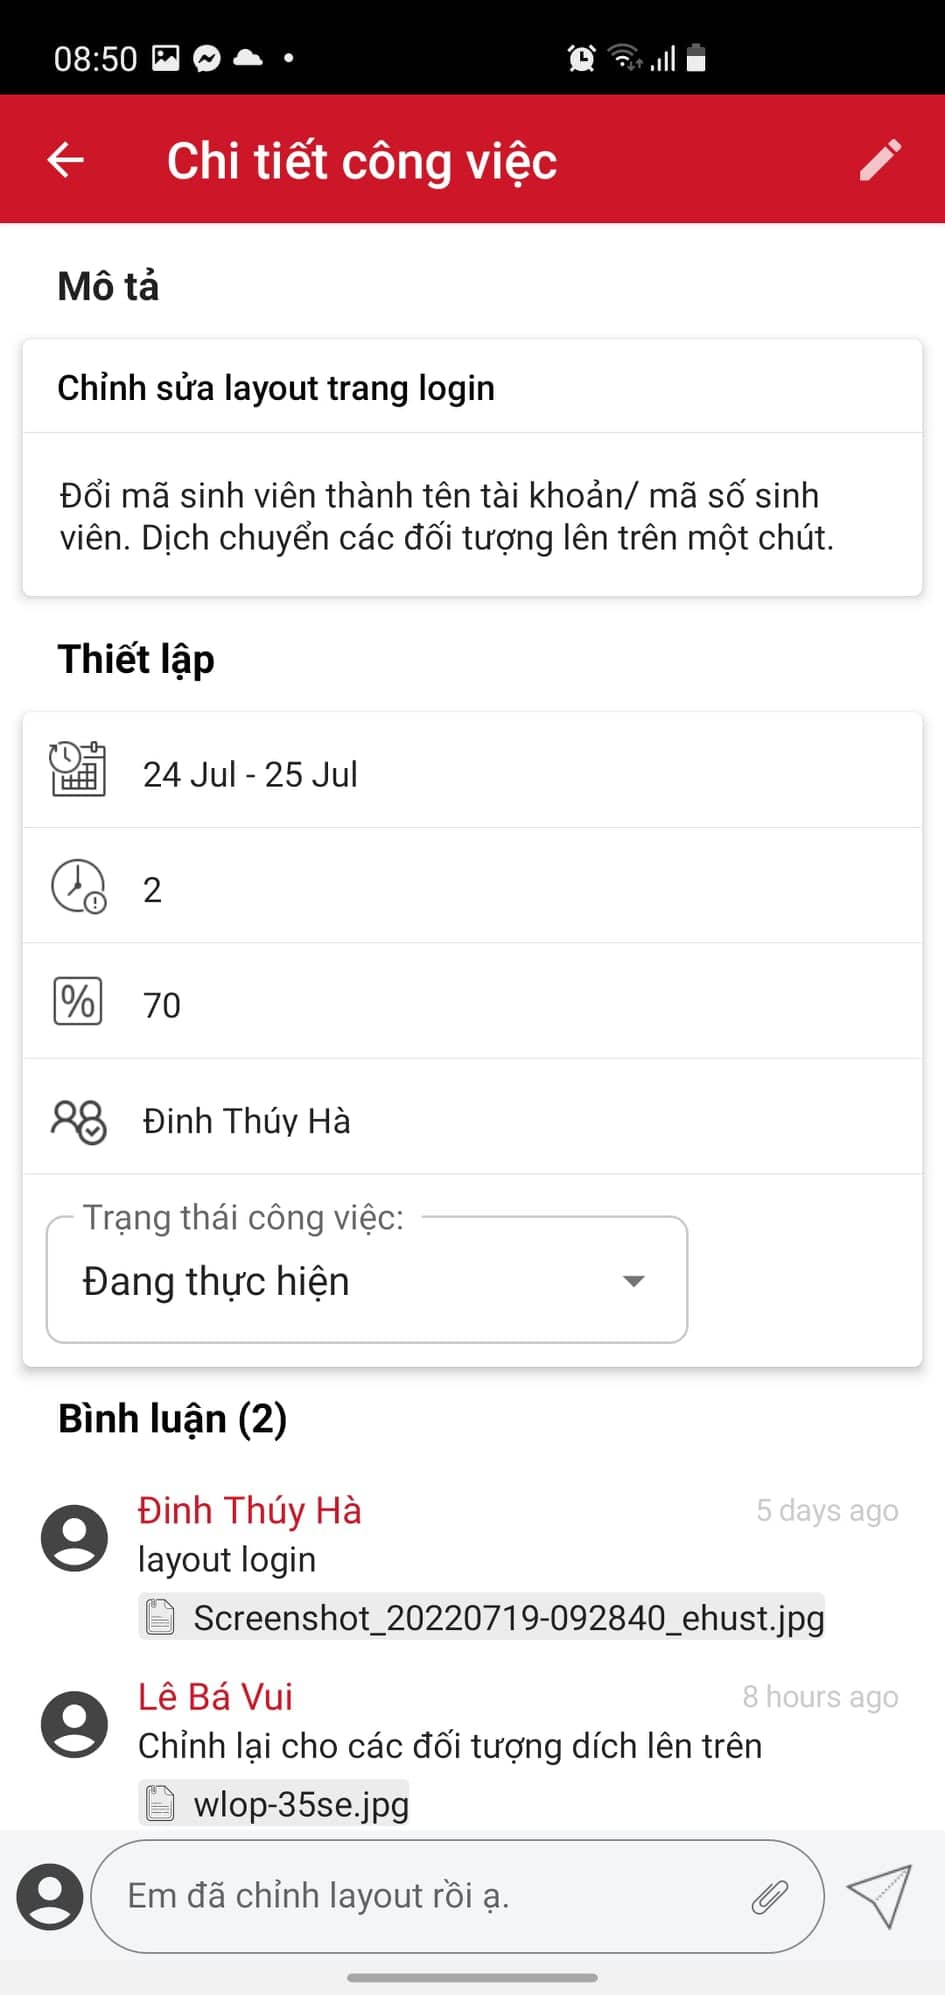
\includegraphics[width=0.7\linewidth]{Figure/screen/comment.jpeg}
\captionof{figure}{Màn hình bình luận công việc} \label{Figure/screen/information_topic.jpeg}
\end{minipage}
\hspace{\fill}
\begin{minipage}{0.5\textwidth}
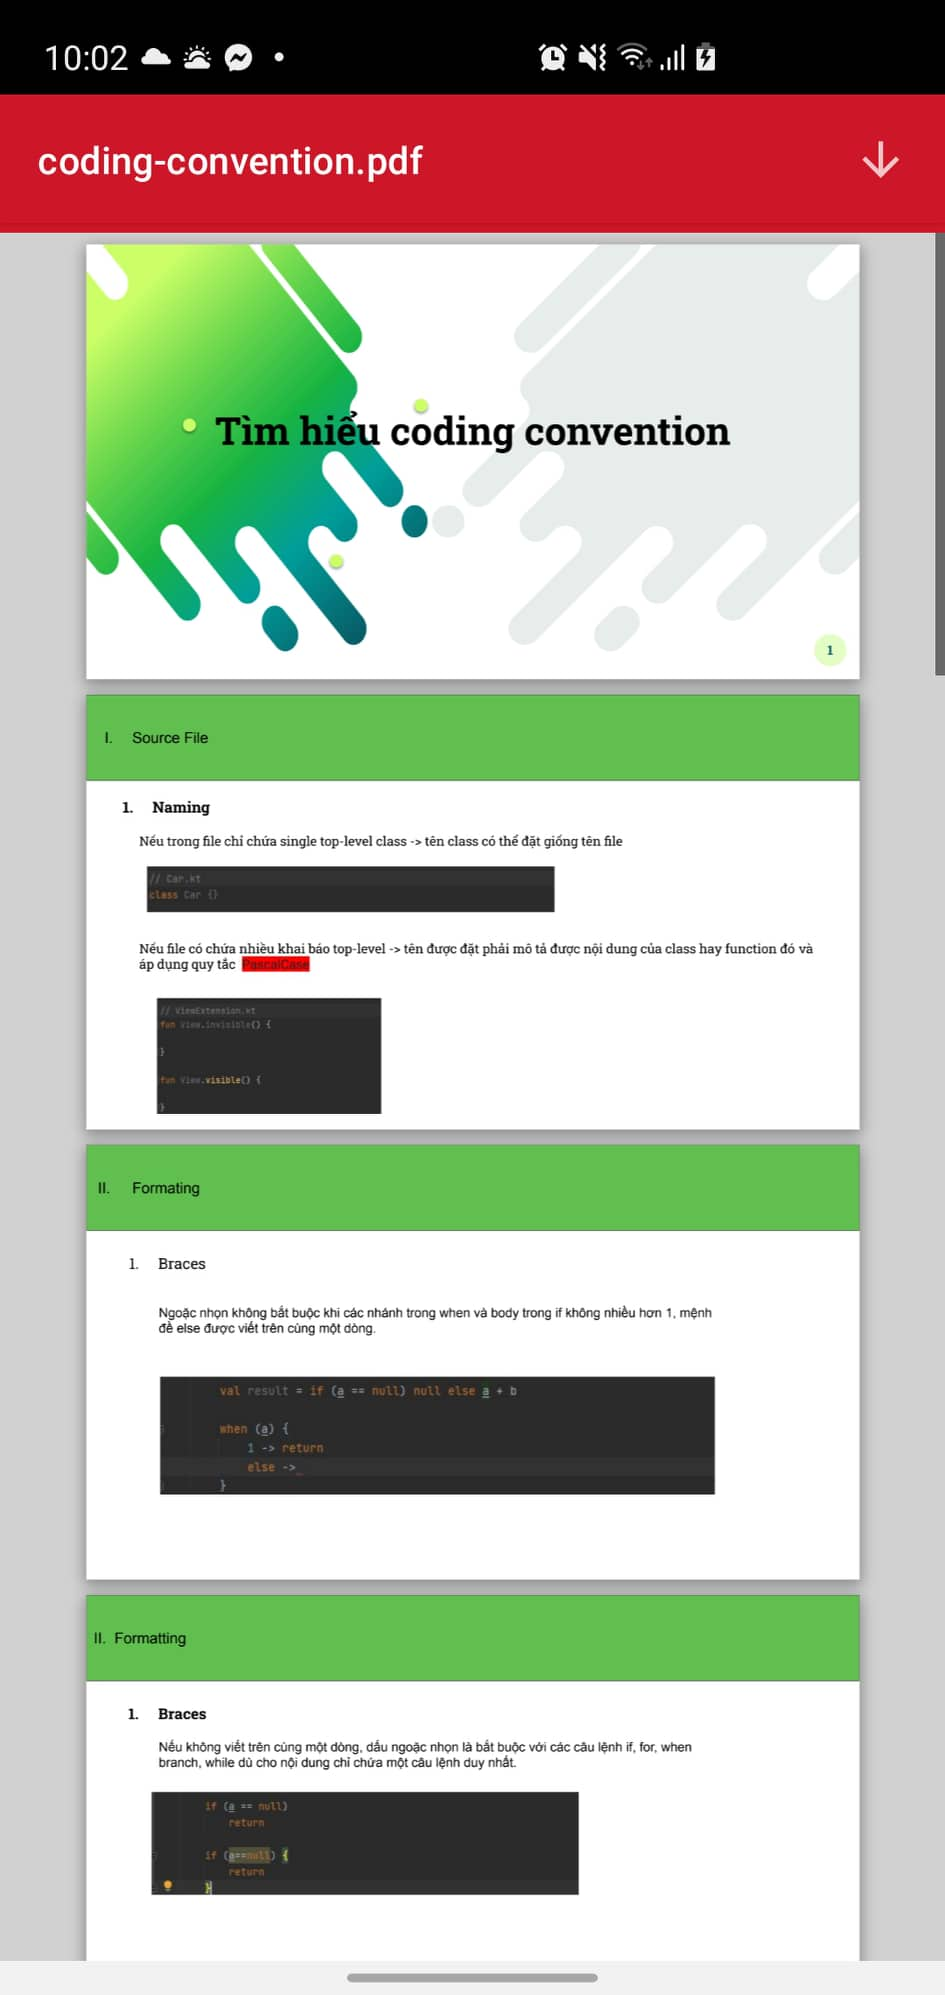
\includegraphics[width=0.7\linewidth]{Figure/screen/show_file_att.jpg}
\captionof{figure}{Màn hình xem file đính kèm} \label{fig:star2}
\end{minipage}

\newpage
\textbf{*Đối với người dùng là sinh viên:}
\begin{figure}[H]
\begin{minipage}{0.5\textwidth}
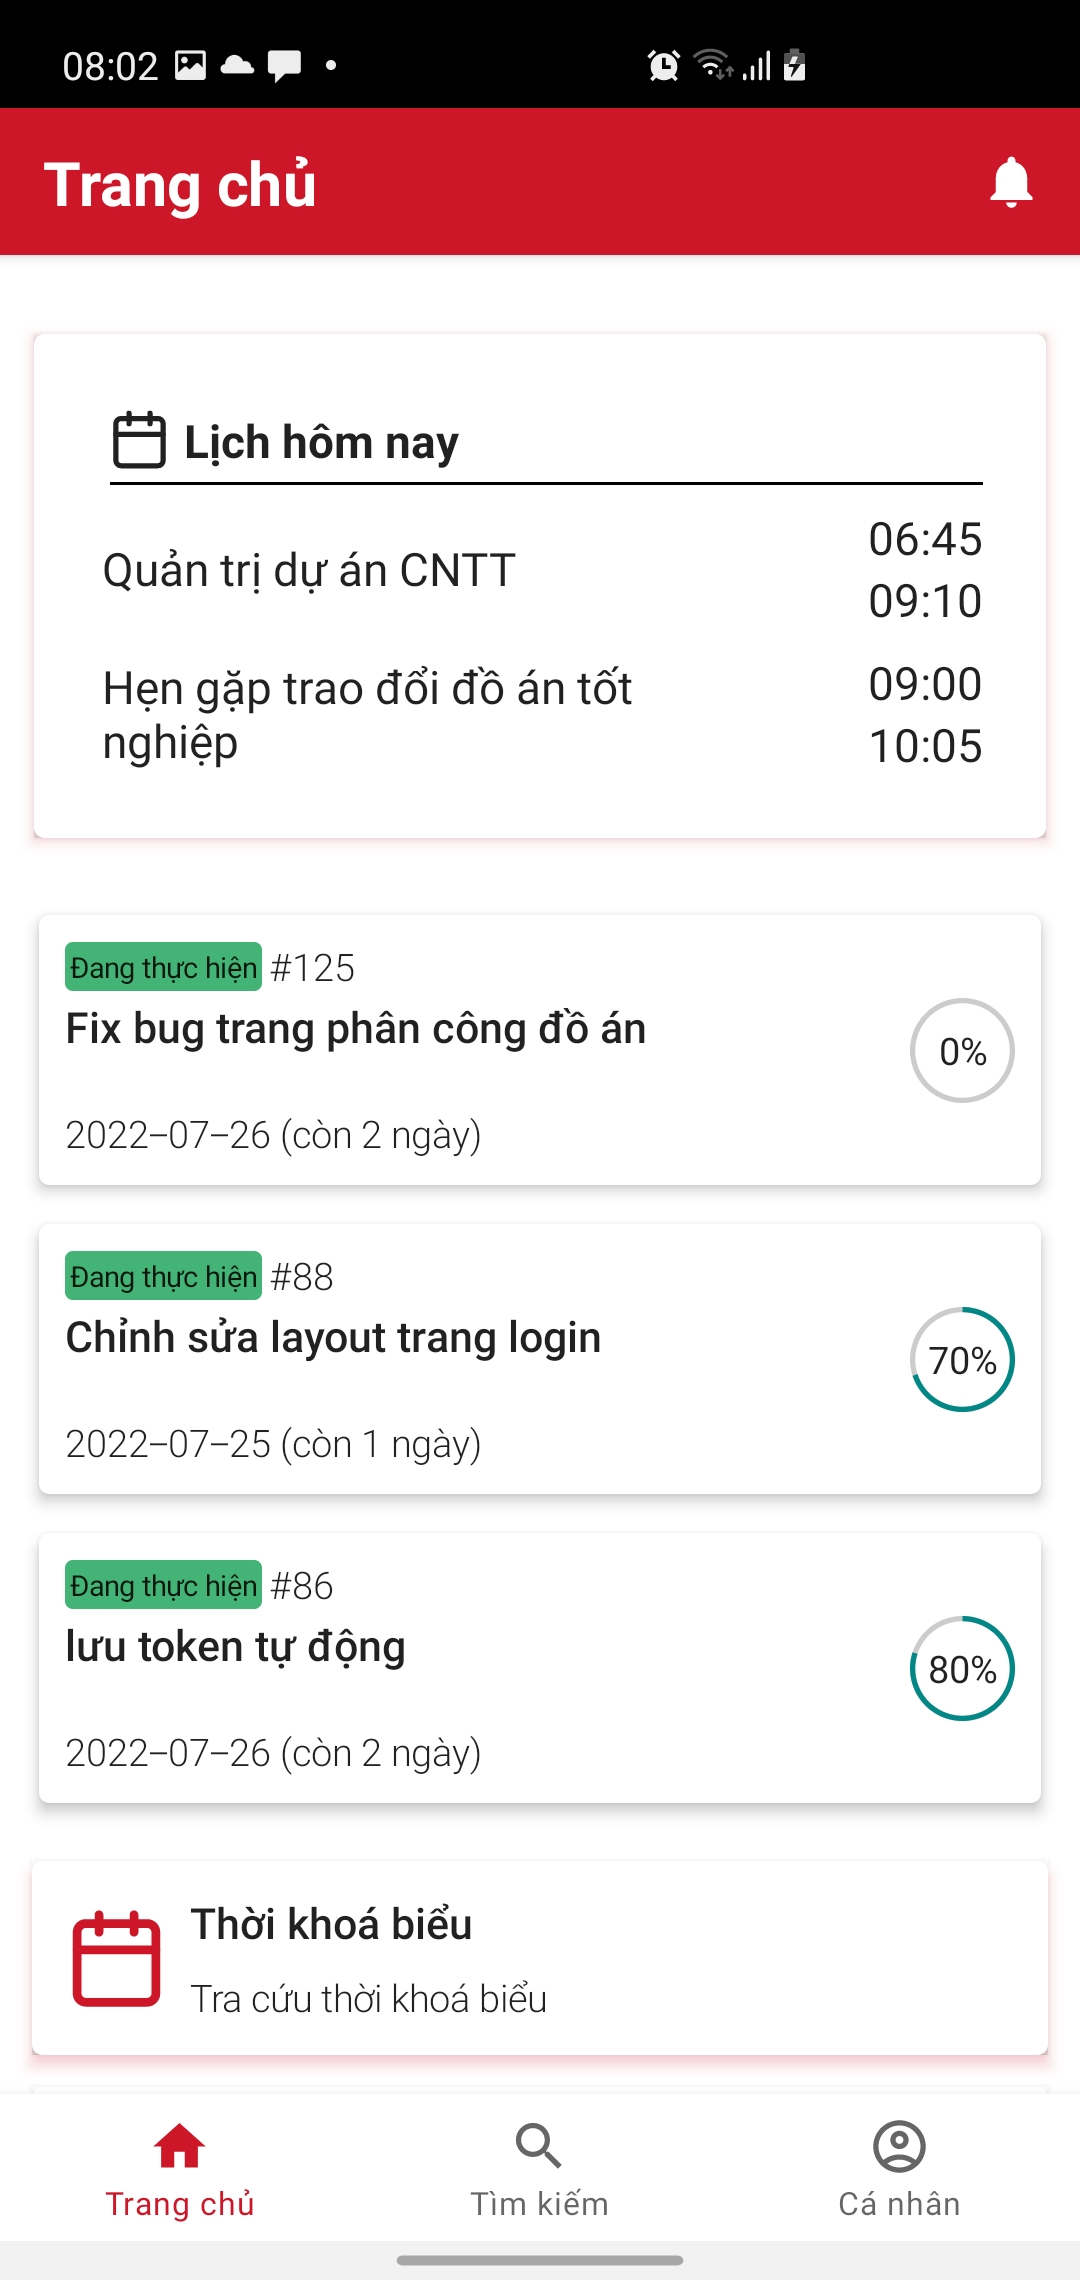
\includegraphics[width=0.60\linewidth]{Figure/screen/home_student.jpg}
\caption{Màn hình trang chủ của sinh viên} \label{fig:screen_login}
\end{minipage}
\hspace{\fill}
\begin{minipage}{0.5\textwidth}
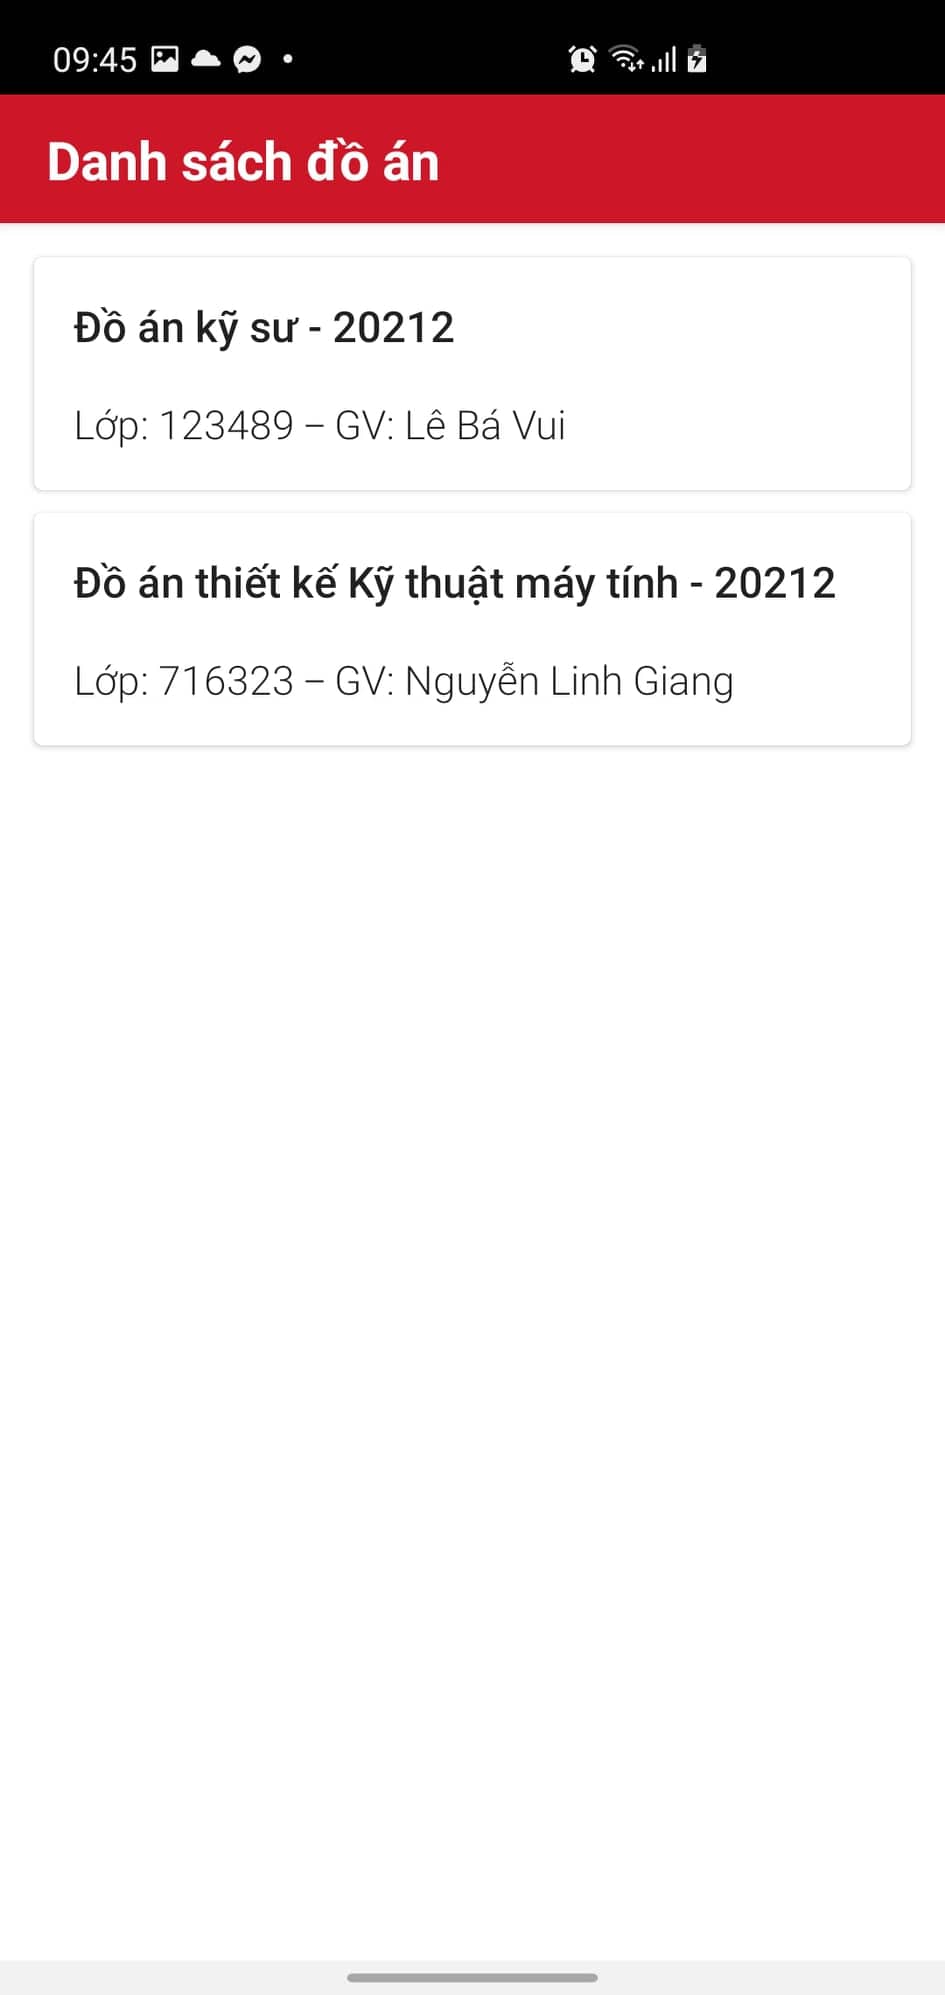
\includegraphics[width=0.60\linewidth]{Figure/screen/ds_project.jpeg}
\caption{Màn hình danh sách đồ án đang làm} \label{fig:list_task}
\end{minipage}
\end{figure}

%% a non-floating version

\textbf{*Đối với người dùng là giảng viên:}

\begin{figure}[H]
\begin{minipage}{0.5\textwidth}
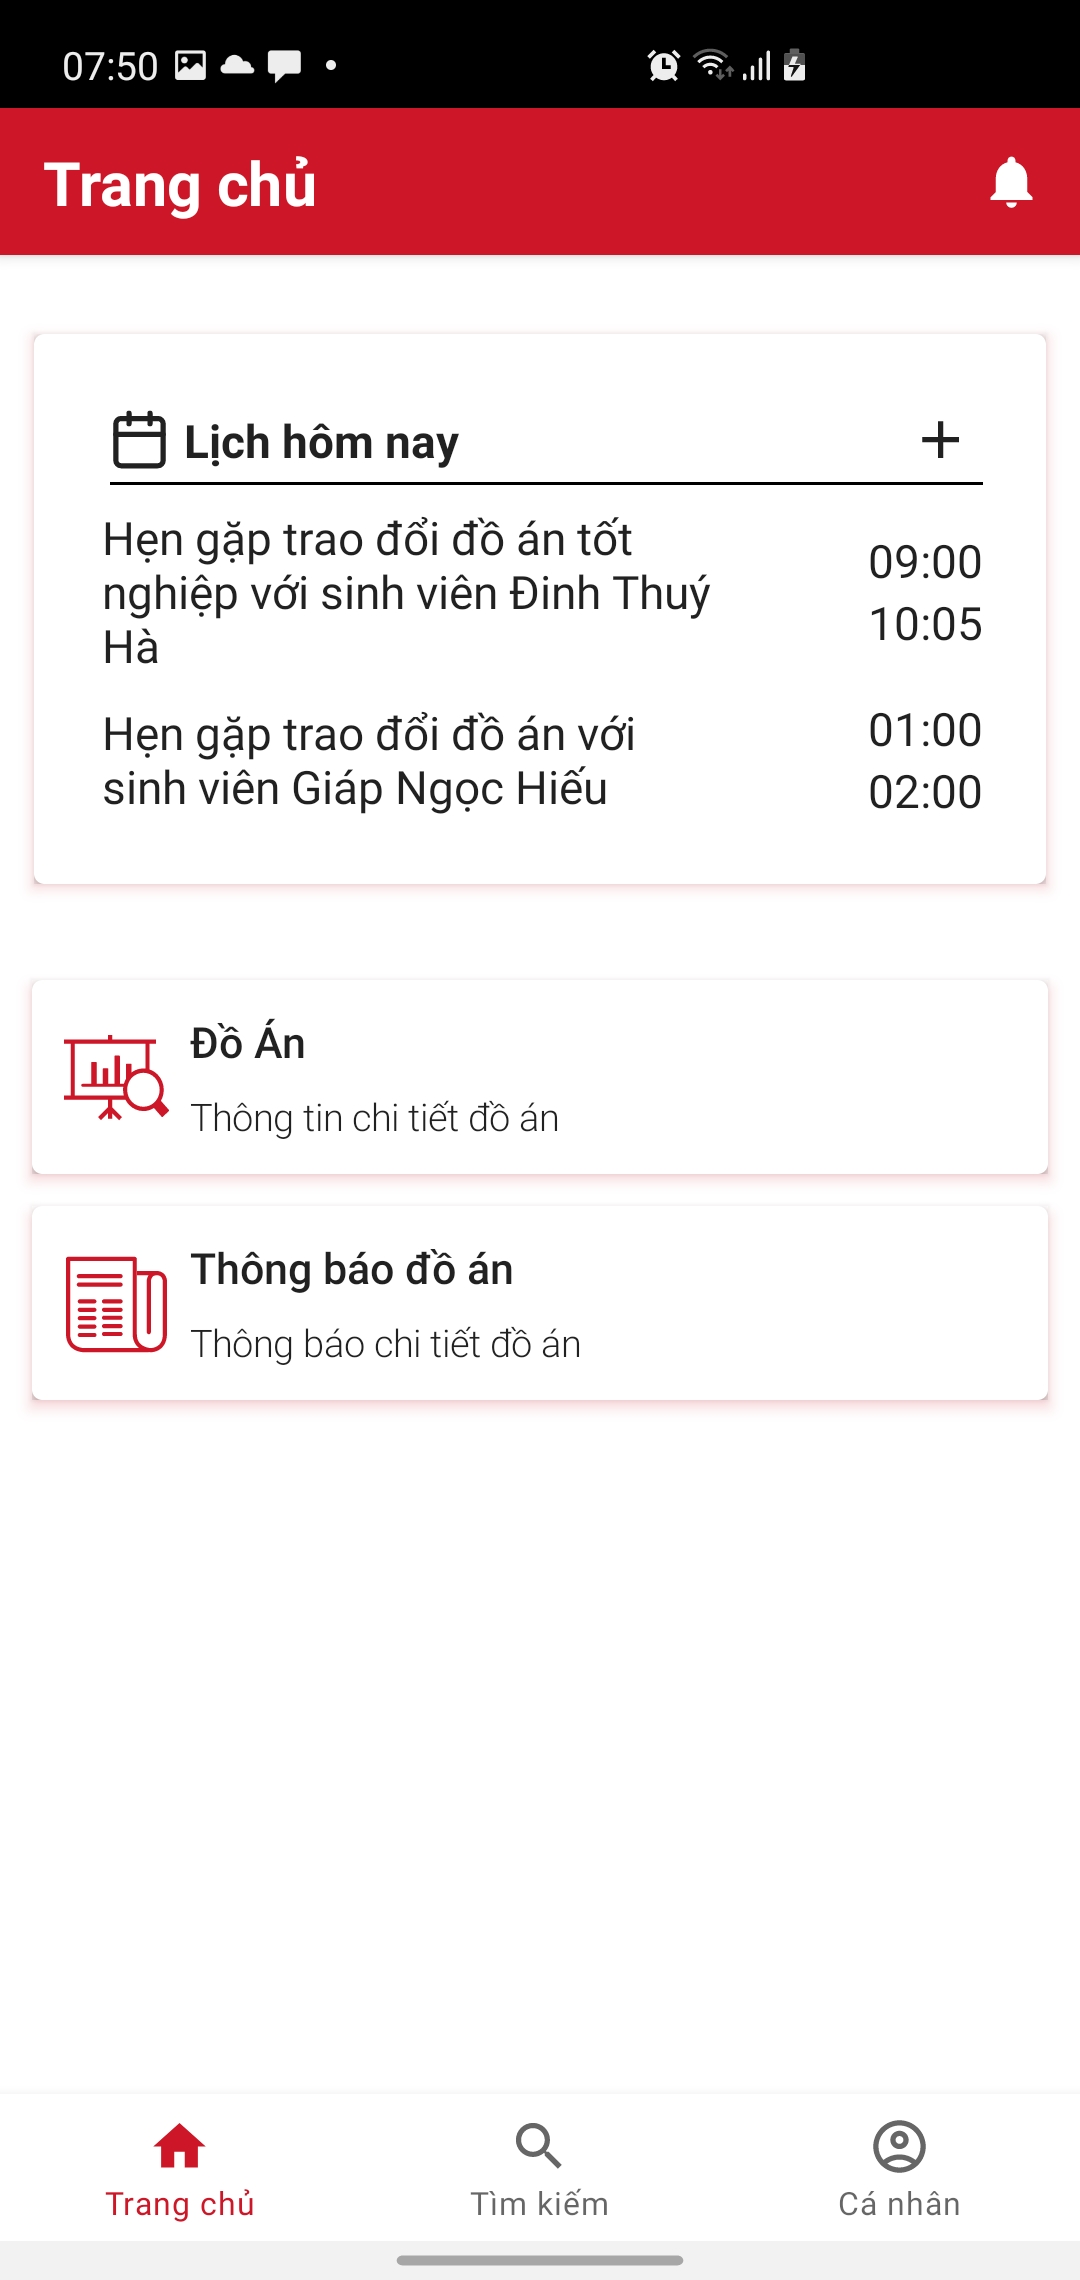
\includegraphics[width=0.60\linewidth]{Figure/screen/screen_home_teacher.jpg}
\caption{Màn hình trang chủ của giảng viên} \label{fig:screen_login}
\end{minipage}
\hspace{\fill}
\begin{minipage}{0.5\textwidth}
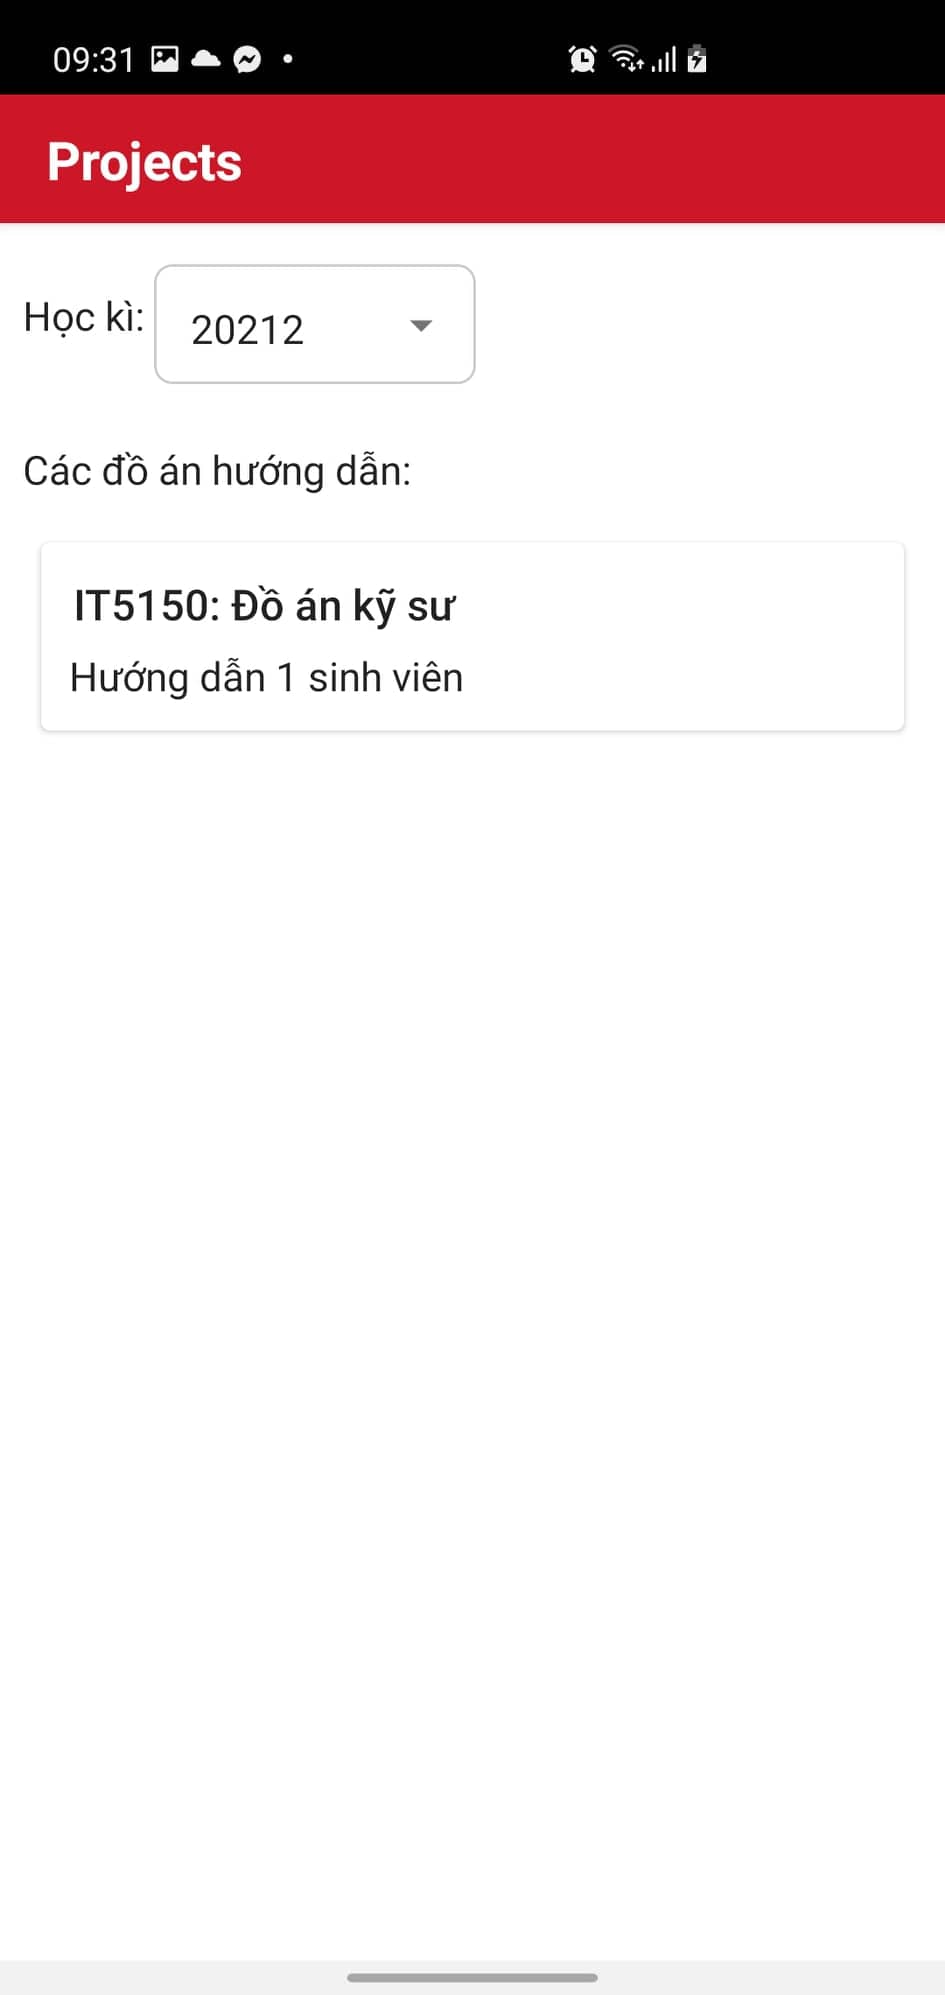
\includegraphics[width=0.60\linewidth]{Figure/screen/project_semester.jpeg}
\caption{Màn hình danh sách đồ án hướng theo học kì} \label{fig:list_task}
\end{minipage}
\end{figure}
\newpage
%% a non-floating version
\noindent %  override any \parindent effect
\begin{minipage}{0.5\textwidth}
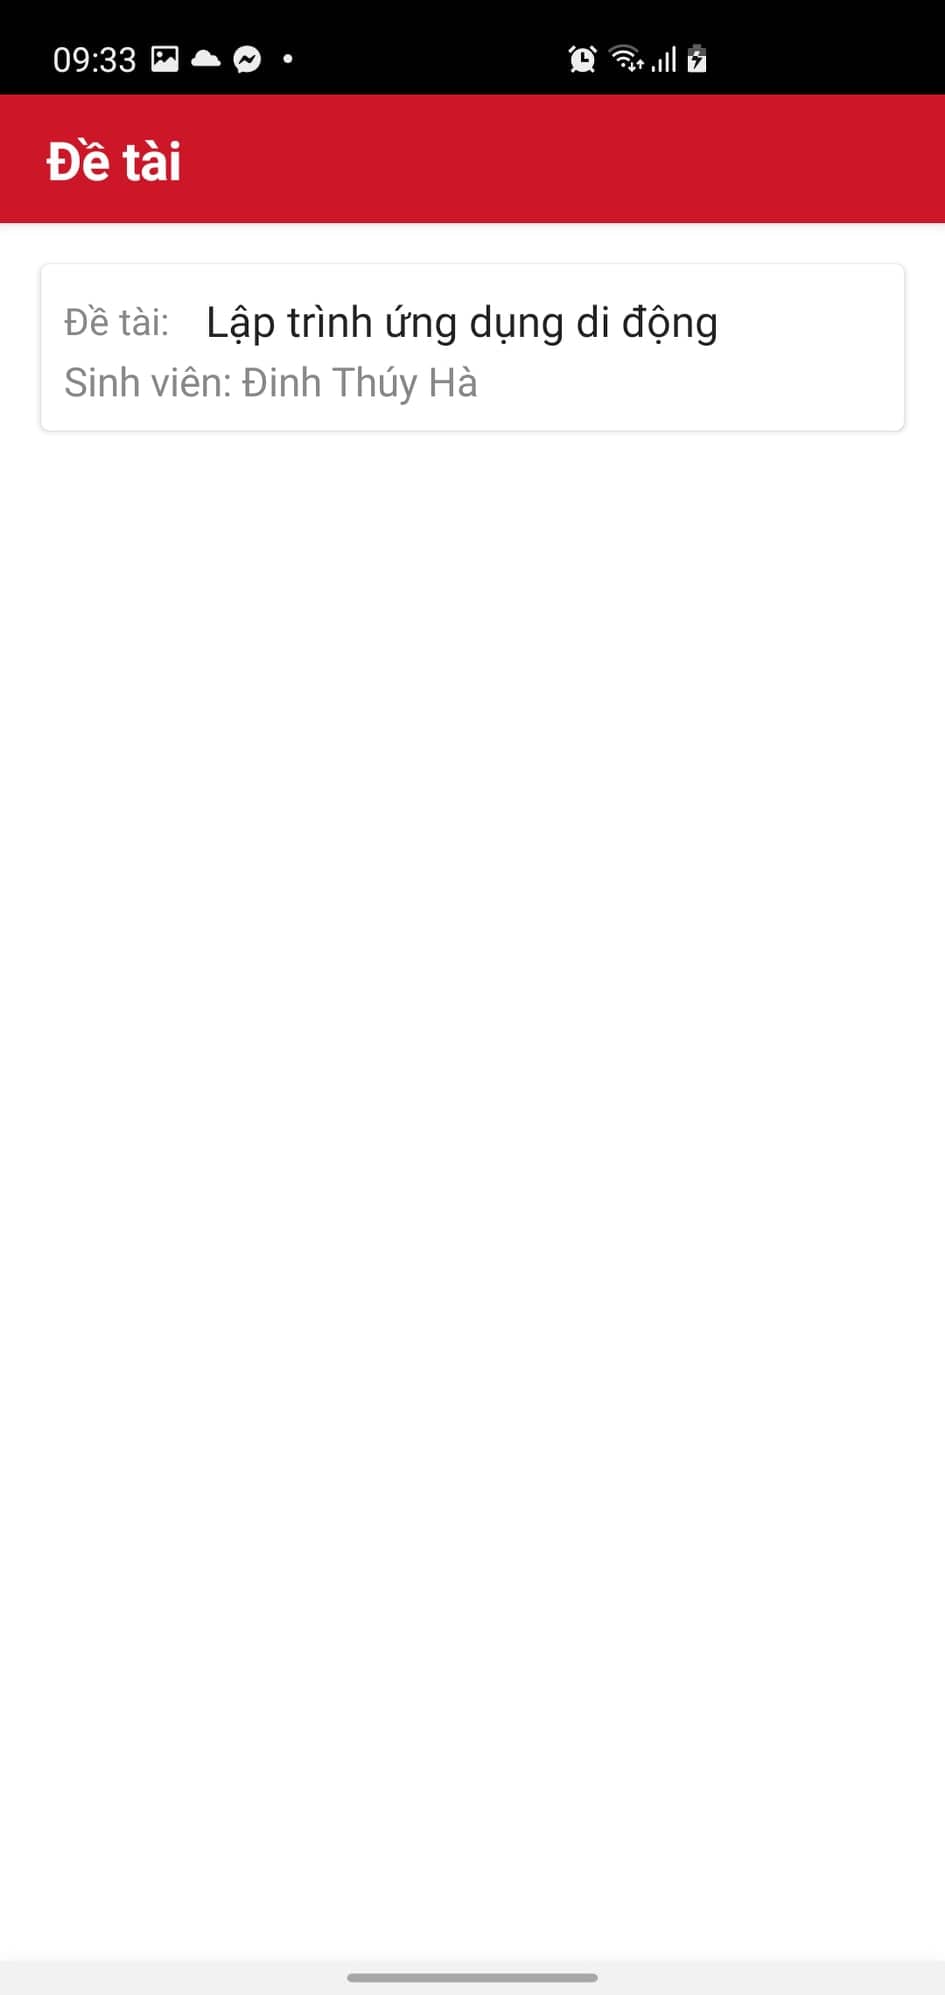
\includegraphics[width=0.67\linewidth]{Figure/screen/ds_de_tai_cua_project.jpeg}
\captionof{figure}{Màn hình danh sách đề tài hướng dẫn của Đồ án kỹ sư} \label{Figure/screen/information_topic}
\end{minipage}
\hspace{\fill}
\begin{minipage}{0.5\textwidth}
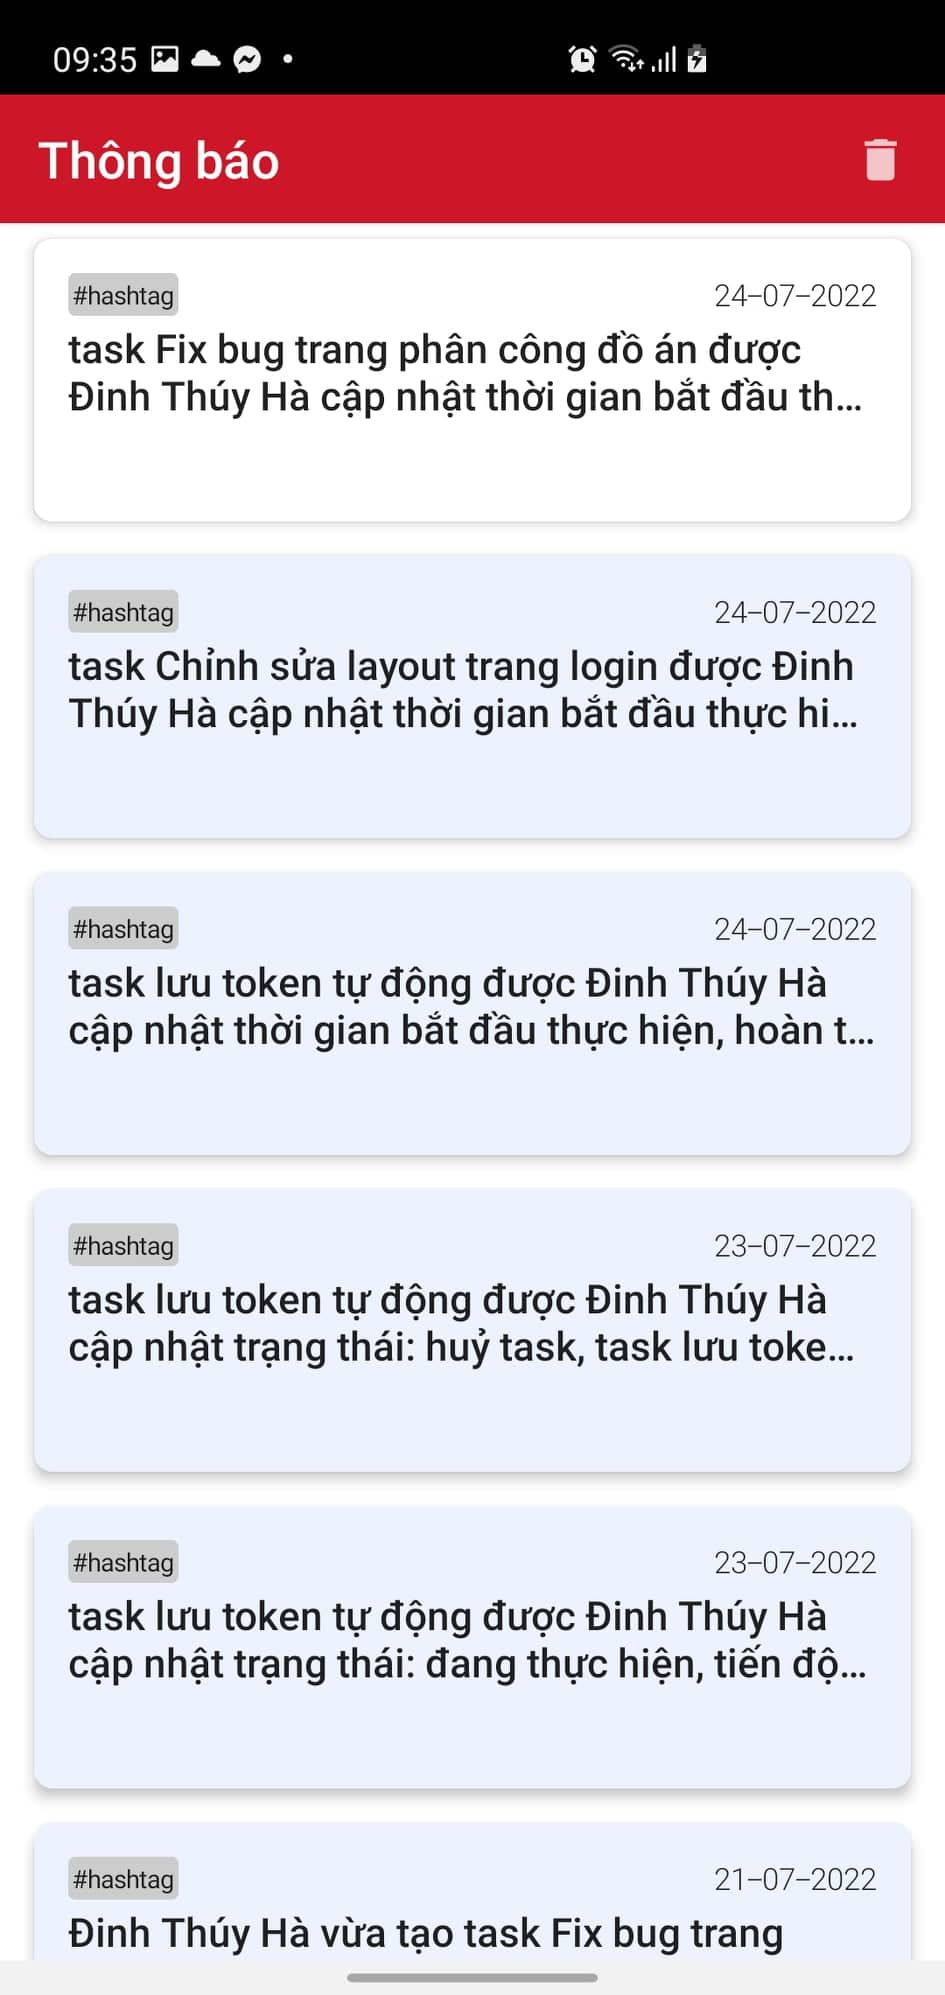
\includegraphics[width=0.67\linewidth]{Figure/screen/information_project.jpeg}
\captionof{figure}{Màn hình danh sách thông báo về đồ án} \label{fig:star2}
\end{minipage}

\begin{figure}[H]
\centering
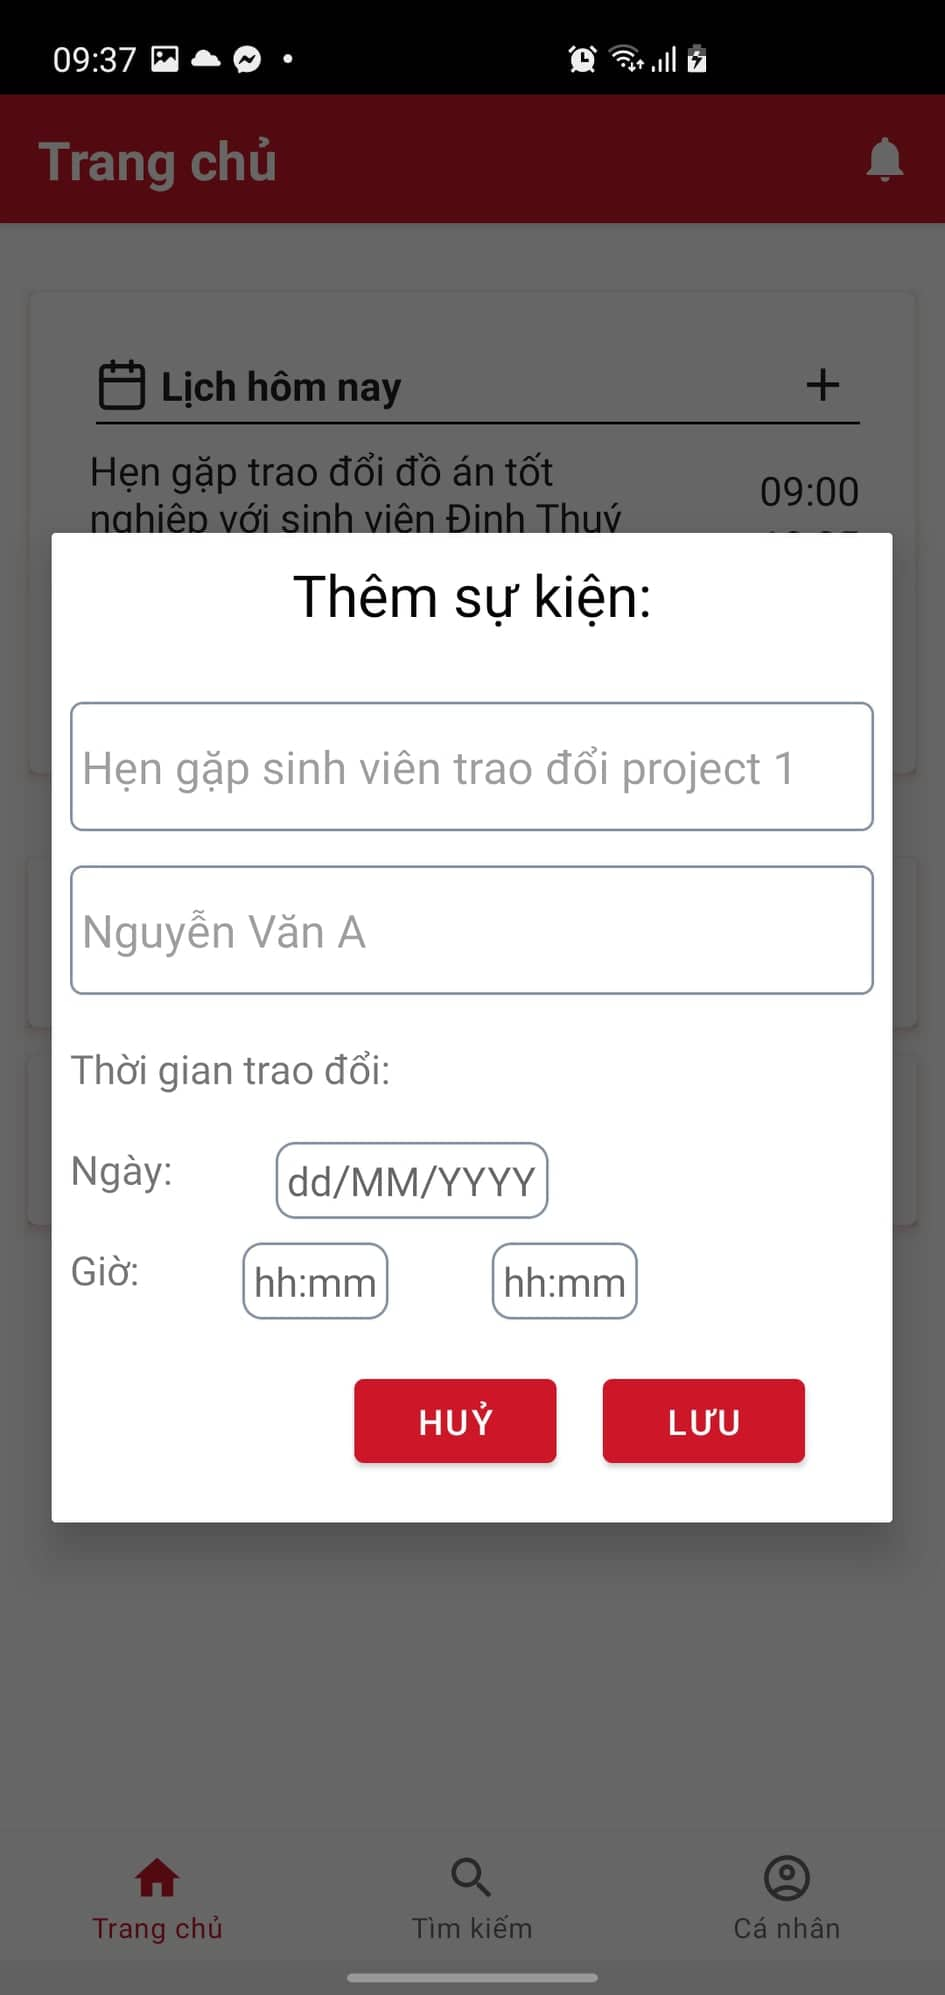
\includegraphics[width=0.35\linewidth]{Figure/screen/new_meeting.jpeg}
\caption{Màn hình tạo lịch gặp sinh viên} \label{fig:screen_login}
\end{figure}

\textbf{*Đối với người dùng là quản trị viên:}

\begin{figure}[H]
\begin{minipage}{0.5\textwidth}
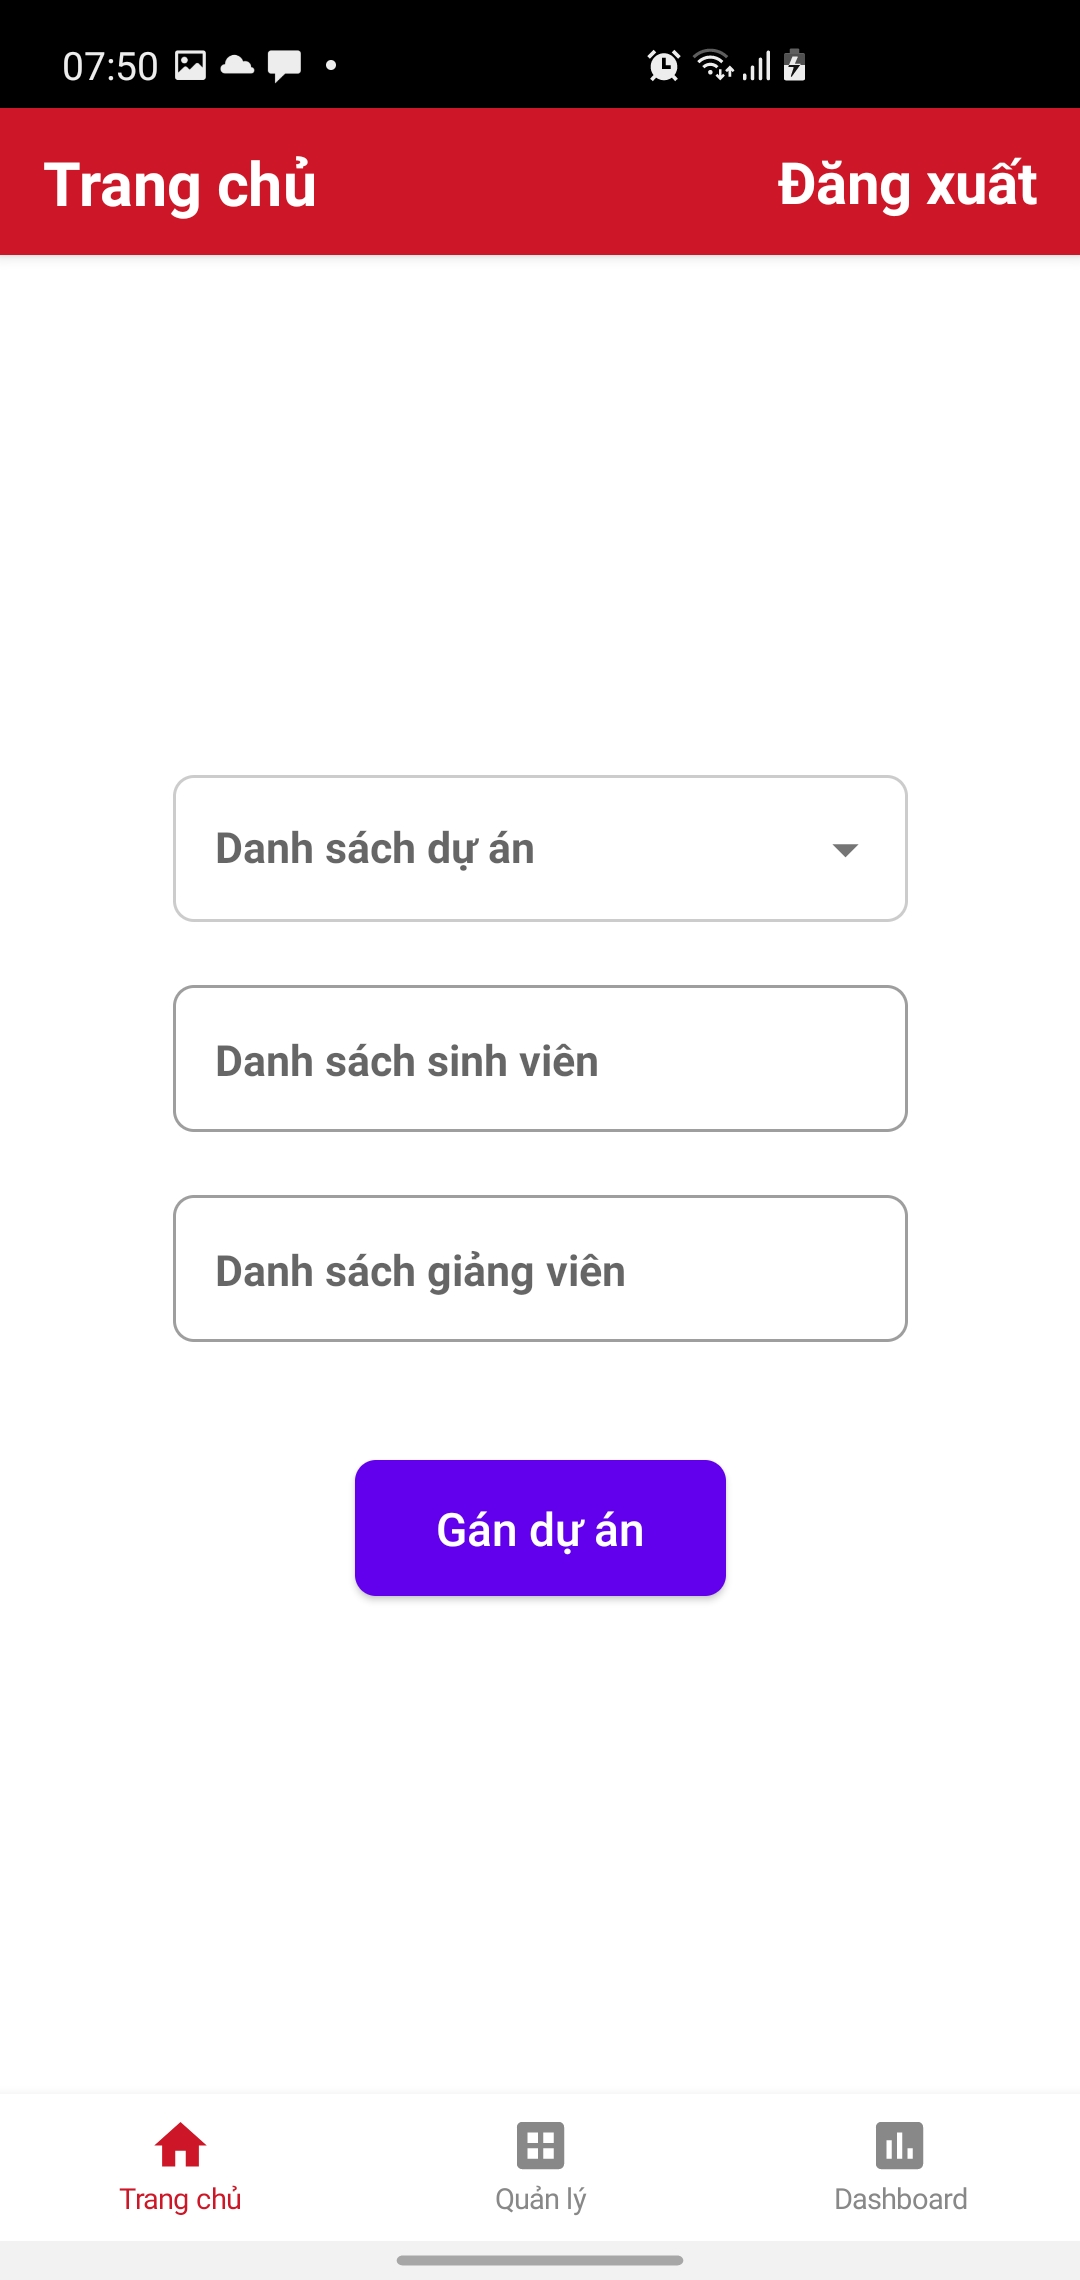
\includegraphics[width=0.66\linewidth]{Figure/screen/screen_home_admin.jpg}
\caption{Màn hình trang chủ của quản trị viên} \label{fig:screen_login}
\end{minipage}
\hspace{\fill}
\begin{minipage}{0.5\textwidth}
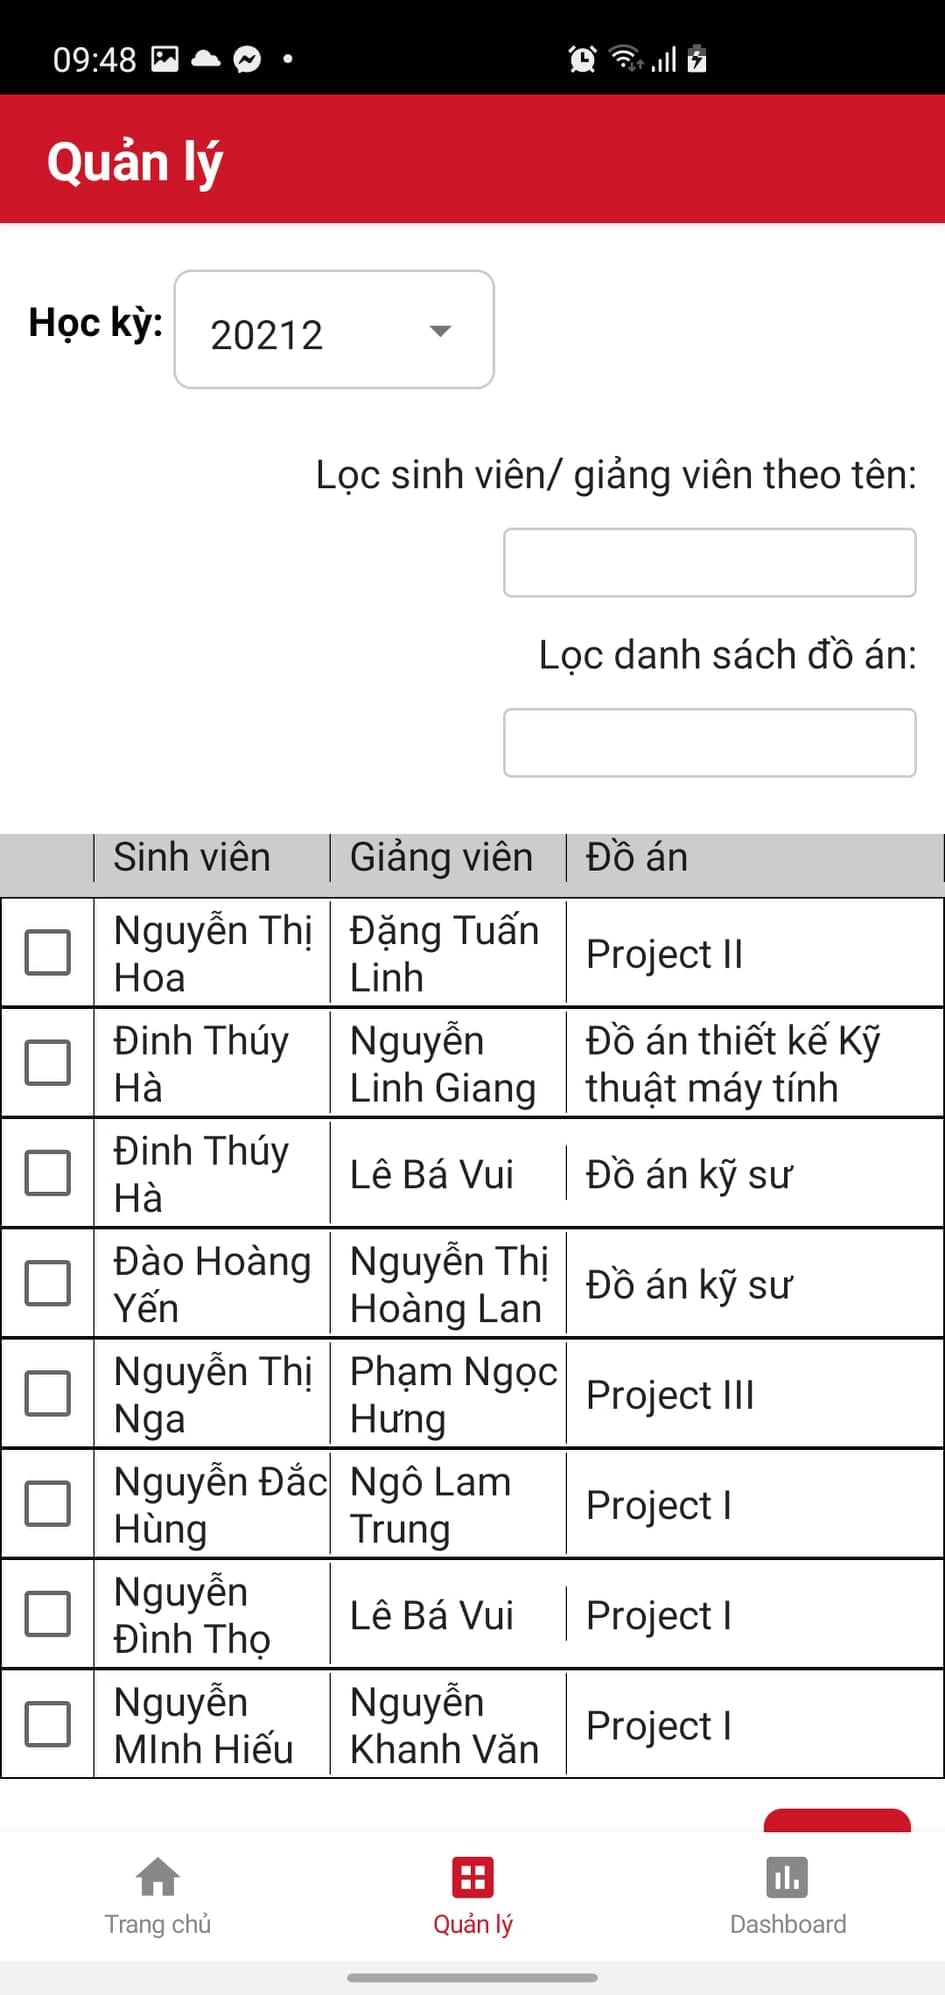
\includegraphics[width=0.66\linewidth]{Figure/screen/management_project.jpeg}
\caption{Màn hình quản lí phân công đồ án} \label{fig:list_task}
\end{minipage}
\end{figure}
%% a non-floating version
\noindent %  override any \parindent effect
\begin{minipage}{0.5\textwidth}
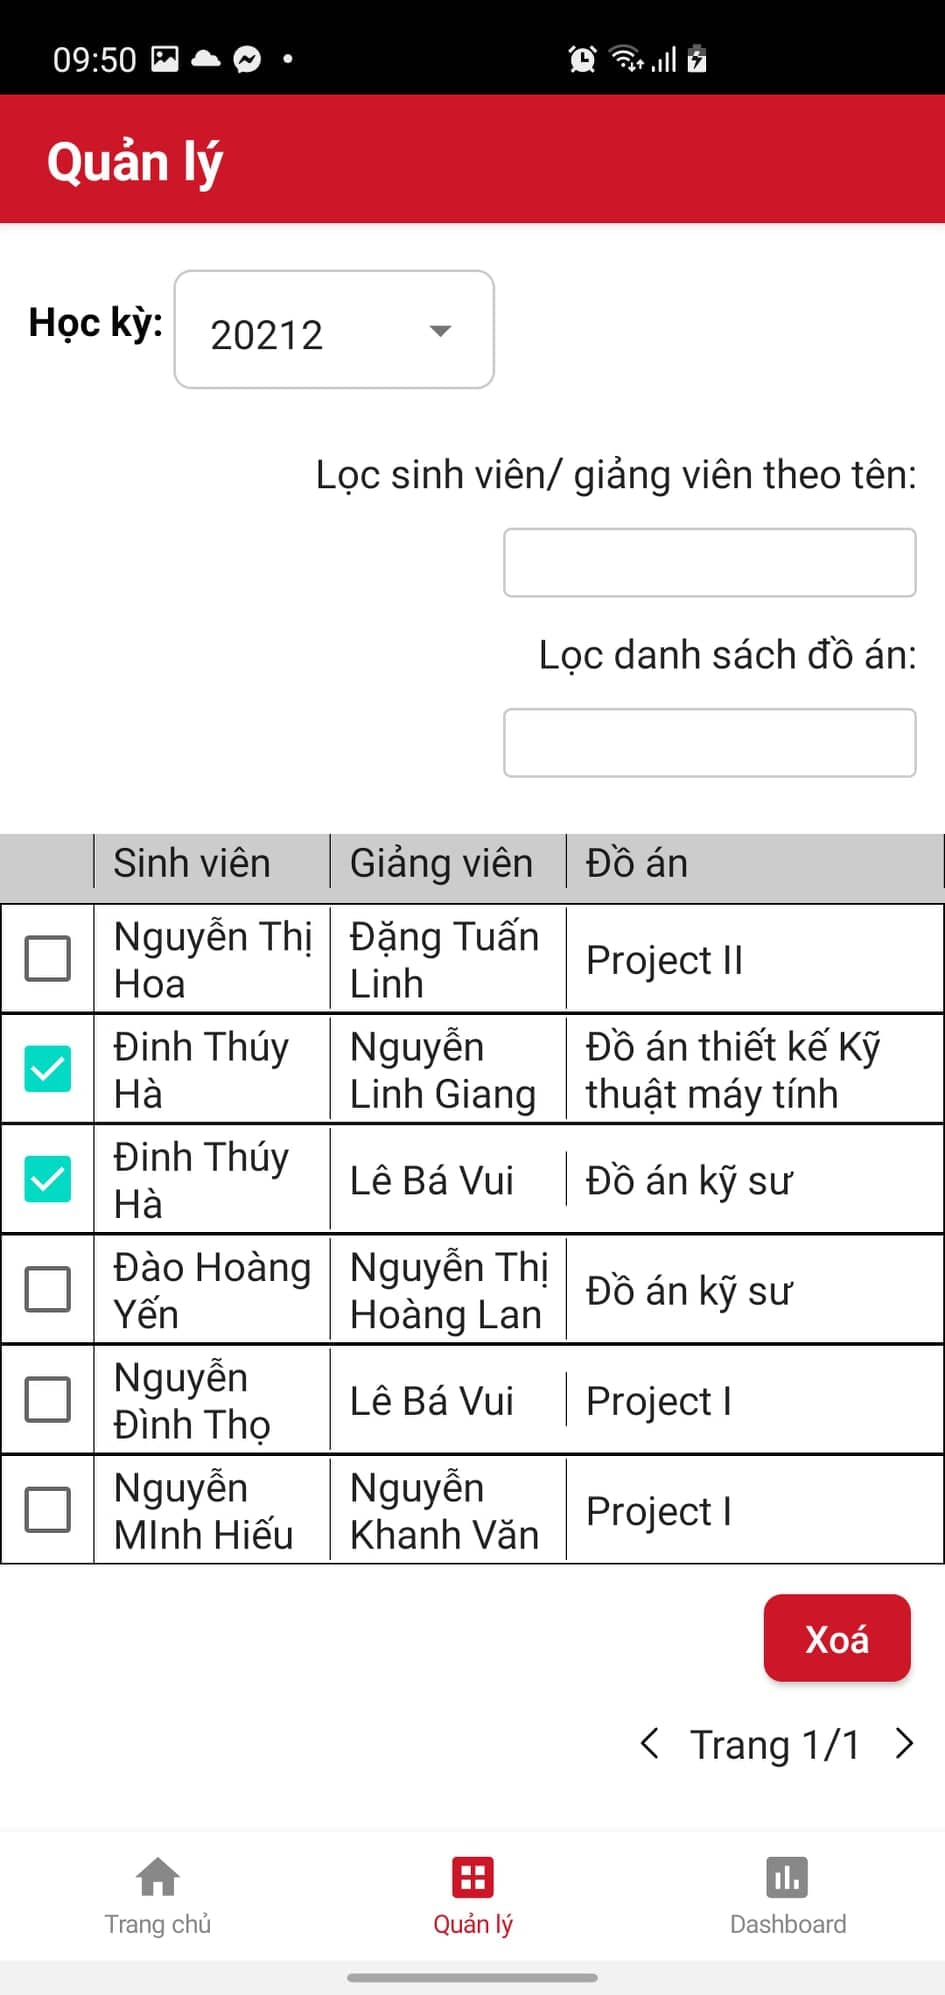
\includegraphics[width=0.66\linewidth]{Figure/screen/delete_assign_1.jpeg}
\captionof{figure}{Màn hình chọn xoá phân công đồ án để xoá} \label{Figure/screen/information_topic}
\end{minipage}
\hspace{\fill}
\begin{minipage}{0.5\textwidth}
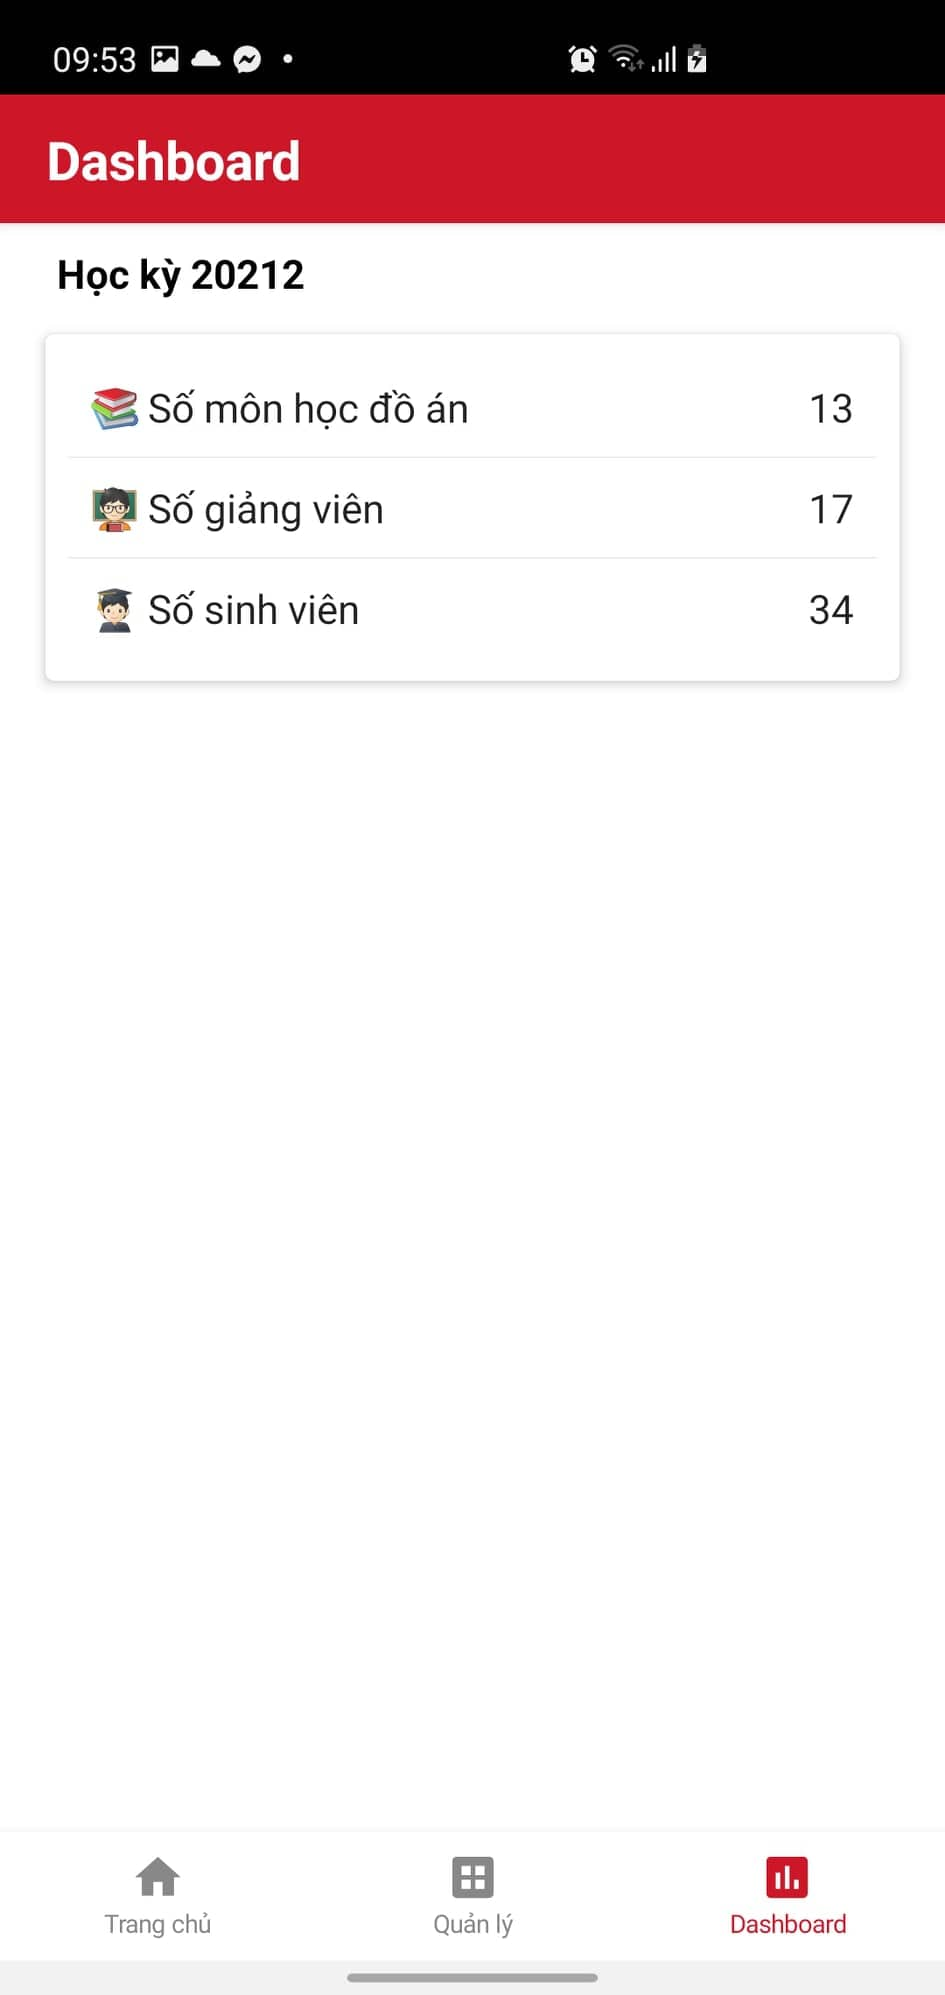
\includegraphics[width=0.66\linewidth]{Figure/screen/dash_board.jpeg}
\captionof{figure}{Màn hình thống kê thông tin} \label{fig:star2}
\end{minipage}

\section{Kiểm thử} 
\begin{table}[H]
\centering
\bgroup
\renewcommand{\arraystretch}{1.5}%
\begin{tabular}{|L{0.06\linewidth}|L{0.15\linewidth}|L{0.3\linewidth}L{0.29\linewidth}|L{0.05\linewidth}|}

\hline
\textbf{STT} & \textbf{Chức năng} & \multicolumn{1}{l|}{\textbf{Đầu vào}} & \textbf{Đầu ra} & \textbf{\begin{tabular}[c]{@{}l@{}}Kết \\ quả\end{tabular}} \\ \hline

\multirow{5}{*}{\linewidth} & \multirow{5}{*}{Đăng nhập} & \multicolumn{1}{L{0.3\linewidth}|}{Điền đầy đủ, hợp lệ thông tin và tài khoản trùng khớp với trong  cơ sở dữ liệu với role\_id = 0} & Đăng nhập thành công và chuyển đến trang chủ của quản trị viên & \multirow{5}{*}{Đạt} \\ \cline{3-4}
1 &  & \multicolumn{1}{L{0.3\linewidth}|}{Điền đầy đủ, hợp lệ thông tin và tài khoản trùng khớp với trong cơ sở dữ liệu với role\_id = 1} & Đăng nhập thành công và chuyển đến trang chủ của giảng viên &  \\ \cline{3-4}
 &  & \multicolumn{1}{L{0.3\linewidth}|}{Điền đầy đủ, hợp lệ thông tin và tài khoản trùng khớp với trong cơ sở dữ liệu với role\_id = 2} & Đăng nhập thành công và chuyển đến trang chủ của sinh viên &  \\ \cline{3-4}
 &  & \multicolumn{1}{L{0.3\linewidth}|}{Điền thiếu một hoặc nhiều trường trong form} & Hiển thị thông báo lỗi &  \\ \cline{3-4}
 &  & \multicolumn{1}{L{0.3\linewidth}|}{Nhập sai thông tin tài  khoản hoặc mật khẩu} & Hiển thị thông báo lỗi &  \\ \hline
2 & Đăng xuất & \multicolumn{1}{L{0.3\linewidth}|}{Chọn Đăng xuất} & Đăng xuất ra khỏi hệ thống và chuyển đến màn hình đăng nhập & Đạt \\ \hline

3 & Xem chi tiết công việc & \multicolumn{1}{L{0.3\linewidth}|}{Chọn một công việc} & Chuyển đến màn hình chi tiết công việc, có đầy đủ các thông tin của công việc & Đạt \\ \hline

4 & Tạo công việc& \multicolumn{1}{L{0.3\linewidth}|}{Chọn button cập nhật ảnh bìa và tải ảnh lên} & Hiển thị bản xem  trước của ảnh bìa khi người dùng tải ảnh lên  sau đó cập nhật lại ảnh bìa và hiển thị cập nhật đó ra trang cá nhân & Đạt \\ \hline
5 & Chỉnh sửa công việc & \multicolumn{1}{L{0.3\linewidth}|}{Điền thông tin vào các trường cần cập nhật} & Cập nhật thông tin thành công và hiển thị thông tin đó lên màn hình& Đạt \\ \hline


\end{tabular}
\egroup

\end{table}
\newpage

\begin{table}[H]
\centering
\bgroup
\renewcommand{\arraystretch}{1.5}%
\begin{tabular}{|L{0.06\linewidth}| 
L{0.15\linewidth}|L{0.3\linewidth}L{0.29\linewidth}|L{0.05\linewidth}|}
\hline
\textbf{STT} & \textbf{Chức năng} & \multicolumn{1}{L{0.3\linewidth}|}{\textbf{Đầu vào}} & \textbf{Đầu ra} & \textbf{Kết quả} \\ \hline
6 & Bình luận công việc & \multicolumn{1}{L{0.3\linewidth}|}{Điền nội dung bình luận, có thể đính kèm file} & Hiển thị bình luận vừa được thêm trên màn hình& Đạt \\ \hline
\multirow{4}{*}{7} & \multirow{4}{\linewidth}{Xem file đính kèm} & \multicolumn{1}{L{0.3\linewidth}|}{Chọn file cần xem nội dung} & Chuyển đến màn hình xem nội dung file & \multirow{4}{*}{Đạt} \\ \cline{3-4}
 &  & \multicolumn{1}{L{0.3\linewidth}|}{Chọn tải file} & Hiển thị thông báo tải file thành công sau khi đã lưu được file về máy &  \\ \cline{3-4}
 &  & \multicolumn{1}{L{0.3\linewidth}|}{Phóng to file} & Nội dung file được phóng to &  \\ \cline{3-4}
 &  & \multicolumn{1}{L{0.3\linewidth}|}{Thu nhỏ file} & Nội dung file được thu nhỏ &  \\ \hline

8 & Xem danh sách thông báo từ trường & \multicolumn{1}{L{0.3\linewidth}|}{Click vào icon thông báo} & Hiển thị danh sách thông báo từ trường & Đạt \\ \hline

9 & Xem danh sách thông báo đồ án & \multicolumn{1}{L{0.3\linewidth}|}{Chọn thẻ thông báo đồ án} & Hiển thị danh sách  thông báo đồ án bao gồm các thông báo đã đọc và chưa đọc & Đạt \\ \hline

10 & Xoá  danh sách thông báo đồ án đã đọc & \multicolumn{1}{L{0.3\linewidth}|}{Chọn icon xoá trên thành actionbar} & Danh sách thông báo đồ án chỉ hiển thị các thông báo chưa đọc& Đạt \\ \hline

\multirow{3}{*}{11} & \multirow{3}{\linewidth}{Tạo lịch gặp sinh viên} & \multicolumn{1}{L{0.3\linewidth}|}{Chọn icon tạo lịch gặp sinh viên} & Mở ra dialog để giảng viên điền thông tin & \multirow{3}{*}{Đạt} \\ \cline{3-4}
 &  & \multicolumn{1}{L{0.3\linewidth}|}{Điền thông tin đầy đủ vào các trường trong dialog, chọn button "OK"} & Ẩn dialog, thông báo tạo lịch gặp thành công &  \\ \cline{3-4}
 &  & \multicolumn{1}{L{0.3\linewidth}|}{Điển thiều một trong các trường, chọn button "OK"} & Thông báo bắt người dùng điền đầy đủ các trường &  \\ \hline

12 & Xem danh sách đồ án hướng dẫn theo kì & \multicolumn{1}{L{0.3\linewidth}|}{Chọn kì học} & Hiển thị danh sách đồ án hướng dẫn theo kì & Đạt \\ \hline

\end{tabular}
\egroup
\end{table}
\newpage

\begin{table}[H]
\centering
\bgroup
\renewcommand{\arraystretch}{1.5}%
\begin{tabular}{|L{0.06\linewidth}|L{0.15\linewidth}|L{0.3\linewidth}|L{0.29\linewidth}|L{0.05\linewidth}|}
\hline
\textbf{STT} & \textbf{Chức năng} & \textbf{Đầu vào} & \textbf{Đầu ra} & \textbf{Kết quả} \\ \hline

13 & Xem chi tiết đề tài& \multicolumn{1}{L{0.3\linewidth}|}{Click button "Chi tiết" trong thẻ đề tài trong màn hình các công việc} & Chuyển đến màn hình thông tin chi tiết đề tài & Đạt \\ \hline

\multirow{2}{*}{14} & \multirow{2}{\linewidth}{Phân công hướng dẫn đồ án} & Chọn đầy đủ các trường trong màn hình phân công đồ án, click button "Phân công" & Thông báo thành công, reset các trường về trạng thái ban đầu& \multirow{2}{*}{Đạt} \\ \cline{3-4}
 &  & Chọn thiếu một trong ba trường, click button "Phân công"& Thông báo mời người dùng phải chọn đầy đủ cả ba trường &  \\ \hline
\multirow{4}{*}{15} & \multirow{4}{\linewidth}{Lọc danh sách phân công đồ án} & Chọn kì học trong danh sách kì học & Trả về danh sách phân công theo kì & \multirow{4}{*}{Đạt} \\ \cline{3-4}
 &  & Chọn một sinh viên trong danh sách sinh viên & Trả về danh sách phân công lọc theo sinh viên &  \\ \cline{3-4}
 &  & Chọn một giảng viên trong danh sách giảng viên & Trả về danh sách phân công lọc theo giảng viên &  \\ \cline{3-4}
 &  & Chọn đồ án trong danh sách đồ án & Trả về danh sách phân công lọc theo tên đồ án &  \\ \hline
16 & Xoá danh sách phân công đồ án & Chọn phân công cần xoá, chọn button "Xoá" & Trả về danh sách phân công không có các phân công đã chọn xoá & Đạt \\ \hline

17 & Xem thống kê tổng số sinh viên đang đăng kí  các môn đồ án, tổng số giảng viên đang quản lí & \multicolumn{1}{L{0.3\linewidth}|}{Chọn tab thống kê} & Trả về màn hình thống kê tổng số sinh viên đang đăng kí các môn đồ án, tổng số giảng viên đang quản lí & Đạt \\ \hline
18 & Tìm kiếm người dùng & \multicolumn{1}{L{0.3\linewidth}|}{Điền id của người dùng.} & Trả về thông tin cơ bản của người dùng: tên, id. hoặc trả về thông báo "Không tìm thấy kết quả phù hợp" & Đạt \\ \hline


\end{tabular}
\egroup
\end{table}

\begin{table}[H]
\centering
\bgroup
\renewcommand{\arraystretch}{1.5}%
\begin{tabular}{|L{0.06\linewidth}|L{0.15\linewidth}|L{0.29\linewidth}L{0.3\linewidth}|L{0.05\linewidth}|}
\hline
\textbf{STT} & \textbf{Chức năng} & \multicolumn{1}{L{0.3\linewidth}|}{\textbf{Đầu vào}} & \textbf{Đầu ra} & \textbf{Kết quả} \\ \hline

19 & Tìm kiếm lớp & \multicolumn{1}{L{0.3\linewidth}|}{Điền mã lớp} & Trả về thông tin lớp: mã lớp, tên môn học, hình thức học, mã lớp, kì học. Hoặc trả về thông báo  "Không tìm thấy kết quả phù hợp" & Đạt \\ \hline

20 & Xem thời khoá biểu & \multicolumn{1}{L{0.3\linewidth}|}{Chọn thẻ thời khoá biểu} & Chuyển sang màn hình xem thời khoá biểu & Đạt \\ \hline
\end{tabular}
\egroup
\caption{Bảng kết quả kiểm thử}
\end{table}
\section{Triển khai}
Backend được triển khai trên Azure Virtual Machine Ubuntu 18.04.6 LTS, backend có thể được sử dụng ở mọi nơi, không cần mất công sức để chạy backend mỗi lần muốn gọi API. Dưới đây là các bước cài đặt và triển khai:

\textbf{Cài đặt:}

Bước 1: Cài đặt Docker
	Sau khi đăng nhập vào máy ảo Ubuntu qua SSH, thực hiện các lệnh sau trên cửa sổ lệnh.

Cập nhật gói:
sudo apt update
sudo apt upgrade

Cài đặt các gói hỗ trợ:
sudo apt-get install curl apt-transport-https ca-certificates software-properties-common

Thêm kho ứng dụng của Docker:
curl -fsSL https://download.docker.com/linux/-\\ubuntu/gpg | sudo apt-key add -

sudo add-apt-repository "deb [arch=amd64] https://download.docker.com/linux- /ubuntu \$(lsb\_release -cs) stable"

sudo apt update

apt-cache policy docker-ce

Cài đặt Docker
sudo apt install docker-ce

Kiểm tra trạng thái dịch vụ Docker đã chạy hay chưa
sudo systemctl status docker

Nếu chưa, có thể khởi động dịch vụ Docker bằng lệnh
sudo systemctl start docker


Bước 2: Cài đặt Nginx
Sau khi đăng nhập vào máy ảo Ubuntu qua SSH, thực hiện các lệnh sau trên cửa sổ lệnh.

sudo apt update
sudo apt install nginx

Kiểm tra trạng thái dịch vụ Nginx đã chạy hay chưa
sudo systemctl status nginx

Nếu chưa, có thể khởi động dịch vụ Nginx bằng lệnh
sudo systemctl start nginx
Bước 3: Cấu hình HTTPS: 

Cài đặt công cụ certbot theo hướng dẫn

https://certbot.eff.org/instructions?ws=nginx\&os=ubuntubionic

Chạy lệnh sau để yêu cầu chứng thư HTTPS và cấu hình với Nginx:
sudo certbot --nginx --register-unsafely-without-email

Nhập tên miền của máy ảo: ehust-vip-pr01.southeastasia.cloudapp.azure.com
	và thực hiện theo hướng dẫn.

Bước 4: Cấu hình nginx
Sau khi đăng nhập vào máy ảo Ubuntu qua SSH, thực hiện các lệnh sau trên cửa sổ lệnh.
		
		cd /etc/nginx/site-enabled

		Chỉnh sửa hoặc tạo mới tệp cấu hình ehust
		sudo nano ehust

		Chỉnh sửa nội dung tệp cấu hình như sau:
\begin{figure}[H]
   \centering
    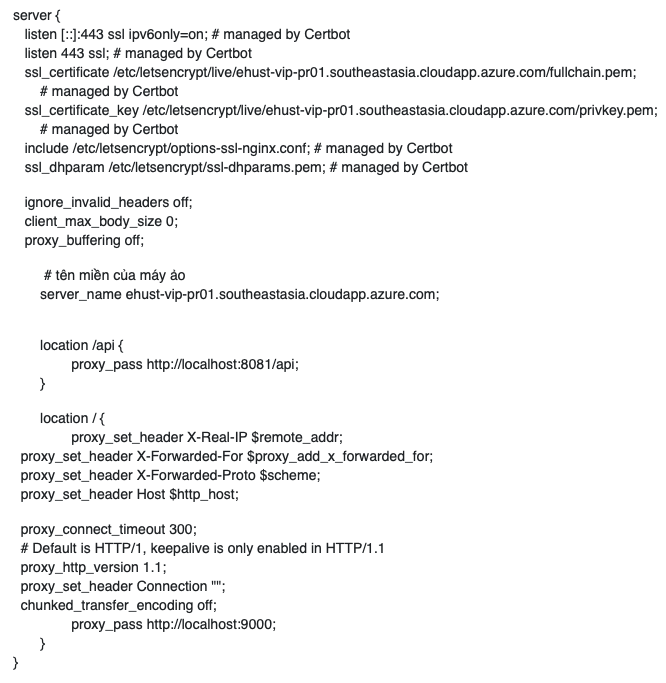
\includegraphics[width=0.85\linewidth]{Figure/cau_hinh_nginx.png}
    \caption{Cấu hình nginx}
    \label{fig:cau_hinh_nginx}
\end{figure}
Lưu tệp cấu hình, sau đó chạy lệnh sau để khởi động lại Nginx
	sudo systemctl reload nginx
 
\textbf{Triển khai:}

Bước 1: Khởi chạy các dịch vụ bằng Docker

Sau khi đăng nhập vào máy ảo Ubuntu qua SSH, thực hiện các lệnh sau trên cửa sổ lệnh.

Chạy container MySQL với lệnh sau:

docker run -d -e MYSQL\_ROOT\_PASSWORD=[*****] -p 127.0.0.1:3306:3306 --name mysql-ins mysql:8

Chạy container Minio với lệnh sau:

docker run -d -p 9000:9000 -p 9001:9001 -e "MINIO\_ROOT\_USER=root" -e "MINIO\_ROOT\_PASSWORD=[*****]" --name minio-ins -v ~/minio-data:/data minio/minio server /data --console-address ":9001"

Tạo dải địa chỉ mạng trong Docker và kết nối với container chạy MySQL:

docker network create ehust-net

docker network connect ehust-net mysql-ins

Bước 2: Tạo tệp thực thi Spring Boot:
Tại máy local, thực hiện lệnh sau trên cửa sổ lệnh tại thư mục gốc của project:

Trên macOS, Linux:
./gradlew build 

Trên Windows:
gradlew.bat build

	Sau khi hoàn tất, tệp thực thi sẽ được lưu tại đường dẫn: ./build/output/ehust-0.0.1-SNAPSHOT.jar

Bước 3: Tạo Docker Image và khởi chạy Spring Boot

Sao chép tệp thực thi ở bước 2 vào máy ảo Ubuntu, tạo tệp định nghĩa Dockerfile với nội dung như sau:

FROM azul/zulu-openjdk-alpine:11-jre

WORKDIR /opt/app

COPY ehust-0.0.1-SNAPSHOT.jar app.jar

CMD ["java", "-jar", "/opt/app/app.jar"]

Tạo Docker Image và chạy container với lệnh sau tại thư mục chứa tệp thực thi và tệp Dockerfile:

docker build -t ehust-app .

docker run -it --name ehust-ins -e SPRING\_PROFILES\_ACTIVE='azure' -d -p 8081:8081 --network ehust-net ehust-app

 Để chạy thử nghiệm Ứng dụng quản lí đồ án chi cần cài đặt thêm APK của ứng dụng.
\end{document}